\documentclass[12pt,a4paper]{article}
\usepackage{color,graphics,amsmath,rotating}

\usepackage{mathrsfs}
\DeclareMathAlphabet{\mathpzc}{OT1}{pzc}{m}{it}


\textheight=24cm
\textwidth=16cm
\oddsidemargin 0cm
\topmargin 0cm
\headsep 0cm
\pagestyle{plain}
\bibliographystyle{unsrt}

\usepackage{color}

\begin{document}

\def\micro{{\tt micrOMEGAs}}
\def\ra{\rightarrow}
\def\calchep{{\tt CalcHEP}}

\def\suspect{{\tt SuSpect}}
\def\mbmb{m_b(m_b)}
\def\mt{m_t}
\def\dMb{\Delta m_b}
\def\dMq{\Delta m_q}
\def\delrho{\Delta\rho}
\def\bsgamma{b\to s\gamma}
\def\bsmu{B_s\to \mu^+\mu^-}
\def\gmuon{(g-2)_\mu}
\def\noi{\noindent}
\def\VERSION{4.2}


\begin{flushright}
   \vspace*{-18mm}
   Date: \today
\end{flushright}
\vspace*{2mm}




\begin{center}


{\Large\bf The  micrOMEGAs user's manual, version 4.1} \\[8mm]

{\large   G.~B\'elanger$^1$, F.~Boudjema$^1$, A.~Pukhov$^2$,  A. Semenov$^3$.}\\[4mm]

{\it 1) LAPTH, Univ. de Savoie, CNRS, B.P.110,  F-74941 Annecy-le-Vieux, France\\
     2) Skobeltsyn Inst. of Nuclear Physics, Moscow State Univ., Moscow 119992, Russia\\
     3) Joint Institute for Nuclear Research (JINR) 141980, Dubna,  Russia\\}
\end{center}

\begin{abstract}
We give an up-to-date description of the micrOMEGAs functions. Only the routines which are available for
the users are described.  Examples on how to use these functions
can be found in the sample main programs distributed with the code. 
\end{abstract}



\tableofcontents

\newpage



\section{Introduction}
\micro~ is a code 
 to calculate the properties of cold dark matter(CDM)  in a generic model of particle physics.  
 First developed to compute the relic density of dark matter, 
 the code also computes the rates for dark matter direct and  indirect detection. 
 \micro~ calculates CDM properties in framework of a model of paricles
 interaction presented in CalcHEP format \cite{Pukhov:2004ca}. 
 It is assumed that the model is invariant ander  a discrete symmetry like R-parity (which is even for 
all standard particles and odd for some new particles including the dark matter candidate) ensures 
the stability of the lightest  odd particle (LOP).  CalcHEP
 package is included in \micro~ and used for matrix elements calculations.
All annihilation and coannihilation channels are included in the computation of the relic density. 
This manual gives an up-to-date description of all \micro~ functions.  
The methods used to compute the different dark matter properties are described 
in references 
~\cite{Belanger:2001fz,Belanger:2004yn,Belanger:2006is,Belanger:2008sj,Belanger:2010gh,Belanger:2013oya}.
These references also contain  a more complete description of the code. In the following
the cold dark matter candidate also called LOP or weakly-interactive massive particle (WIMP)
will be denoted by $\chi$. 

\micro~ contains both C and Fortran routines. Below we describe only the
C-version of the routines,  in general we use the same  names
 and the same types of argument for both  C and Fortran functions. 
We always use \verb|double(real*8)| variables for float point numbers and 
\verb|int(INTEGER)| for integers. In this manual we use {\it FD} for  file descriptor 
variables, the file descriptors  are  \verb|FILE*| in C and {\tt channel number} in Fortran. 
The symbol \verb|&| before the names of variables in C-functions stands for 
the address of the variable. It is used for  {\it output
parameters}. In Fortran calls there is no need for \verb|&|
since  all parameters are passed via addresses. In C programs one  can substitute {\tt
NULL} for any output parameter which the user chooses to ignore. In Fortran  one
can substitute {\tt cNull, iNull, r8Null} for unneeded
parameters of  {\it character}, {\it integer}  and {\it real*8}  type respectively.  

A few C-functions use pointer variables that specify an {\it address} in 
the computer memory. Because pointers do not exist in  Fortran one uses any
other type of variable whose length is sufficient to store a computer address, for example {\it INTEGER*8}.
% array with length 2 or a {REAL*8} variable. 

The complete format  for all functions can be found in
\verb|sources/micromegas.h| (for C) or
\verb|sources/micromegas_f.h| (for Fortran). Examples on how to use these functions are provided   
in the MSSM/main.c[F] file. 
 
\section{Discrete symmetry in \micro.}

 \micro~ exploits the fact that models of dark matter exhibit a discrete symmetry
and that the fields  of the model transform as 
$   \phi \to e^{i2\pi X_{\phi}} \phi$
where the charge $|X_{\phi}|<1$. 
The particles of the  Standard Model 
are assumed to transform trivially under the discrete symmetry, $X_\phi=0$. In the following all particles with
 charge $X_\phi\neq 0$  will be called 
 {\it odd} and the  lightest odd particle  will be  stable. If neutral, it can be considered as a DM candidate.
Typical  examples  of discrete symmetries used for constructing single DM models  are $Z_2$ and  $Z_3$. 
Multi-component DM can arise in models with larger discrete symmetries. A simple 
example is a model with  $Z_2\times Z_2'$ symmetry, the particles charged under  $Z_2$($Z_2'$) will belong to the first (second) dark sector. The lightest particle of each sector  will be stable and therefore a potential DM candidate. 
Another example is a model with a $Z_4$  symmetry.  The two dark sectors contain particles with $X_\phi=\pm 1/4$ and $X_\phi=1/2$ respectively. The lightest particle with  charge $1/4$ is always stable while the lightest particle of charge $1/2$ is stable only if its decay into two particles of charge $1/4$ is kinematically forbidden.
 \micro~ assumes that all odd particles have  names
starting with '\verb|~|', for example, \verb|~o1| for the lightest  
neutralino. In versions 4.X, to distinguish the particles with different transformation properties with 
respect to the discrete group, that is particles belonging to different 'dark' sectors,
we use the convention that the names of particles in the second 'dark' sector starts with '\verb|~~|'. 
Note that \micro~ does not check the symmetry of the Lagrangian, it assumes that the name convention 
correctly identifies  all particles with the same discrete symmetry quantum numbers.

  
\section{Downloading and compilation of micrOMEGAs.}
To   download  micrOMEGAs, go to    \\  
\verb|     http://lapth.cnrs.fr/micromegas|\\
and unpack the file received, \verb|micromegas_|\VERSION\verb|.tgz|, with the command\\
\verb|     tar -xvzf micromegas_|\VERSION\verb|.tgz|\\
This should create the directory \verb|micromegas_|\VERSION\verb|/| which occupies about 40
Mb of disk space. You will need more disk space after compilation of
specific models and generation of matrix elements.
In case of problems and questions\\
\verb|     email: micromegas@lapth.cnrs.fr|\\


\subsection{File structure of micrOMEGAs.}
\label{file_structure}
\verb|Makefile            |  to compile the kernel of the package               \\
\verb|CalcHEP_src/        |        generator of matrix elements for micrOMEGAs    \\
\verb|Packages/        |        external codes    \\
\verb|clean           | to remove compiled files \\
\verb|man/|         |   contains the manual: description of micrOMEGAs routines \\
\verb|newProject          |     to create a new model directory   structure                           \\
\verb|sources/            |        micrOMEGAs code                               \\
{\it MSSM model directory}                                                          \\
\verb|MSSM/               |                                                      \\
\verb|   Makefile         |  to compile the code and executable for  this model \\
\verb|   main.c[pp] main.F|       files with sample {\it main} programs      \\
\verb|   lib/             |      directory for routines specific to this model   \\
\verb|       Makefile     |   to compile the auxiliary code library {\it lib/aLib.a}    \\
\verb|       *.c *.f      |      source codes of auxiliary functions             \\
\verb|   work/            |              CalcHEP working directory for the generation of   \\
\verb|                    |             matrix elements                                    \\
\verb|       Makefile     |  to compile the library {\it work/work\_aux.a}           \\ 
%\verb|       work_aux.a   | information about  parameters and particles.      \\
% \verb|  |{\it Directories for CalcHEP sessions for generation of matrix elements}\\
\verb|       models/      | directory for files  which specifies the model\\ 
\verb|         vars1.mdl  |  free  variables   \\
\verb|         func1.mdl  |  constrained variables   \\
\verb|         prtcls1.mdl|  particles  \\
\verb|         lgrng1.mdl |   Feynman rules\\
\verb|       tmp/         | auxiliary directories for CalcHEP sessions    \\
\verb|       results/  |                                                  \\
\verb|       so_generated/|   storage  of  matrix elements generated by CalcHEP \\
\verb|    calchep/        |   directory for interactive CalcHEP sessions    \\
{\it Directories of other models which have the same structure as} {\tt  MSSM/ }\\
\verb| NMSSM/             |         Next-to-Minimal Supersymmetric Model\cite{Ellwanger:2006rn,Belanger:2005kh} \\
\verb| CPVMSSM/           |         MSSM with complex parameters\cite{Lee:2003nta,  Belanger:2006qa} \\
\verb| IDM/               |         Inert Doublet Model\cite{Barbieri:2006dq}  \\
\verb| LHM/               |         Little Higgs Model\cite{Belyaev:2006jh} \\
\verb| RHNM/              |         Right-handed Neutrino Model\cite{Belanger:2007dx}                  \\
\verb| SM4/               |            Toy model with a 4th generation of lepton and neutrino DM   \\
\verb| Z3M/               |           A model with scalar DM and $Z_3$ discrete
symmetry|\cite{Belanger:2012vp,Belanger:2014bga} \\
\verb| Z4ID/              |           A model with $Z_4$
symmetry|\cite{Belanger:2012vp,Belanger:2014bga} \\  
\verb| mdlIndep/          |           For model independent computation of DM signals                                 \\

\subsection{Compilation of CalcHEP and micrOMEGAs routines.}
   CalcHEP and micrOMEGAs are compiled by {\it gmake}. Go to the micrOMEGAs directory
and launch\\
\verb|     gmake|\\
If {\tt gmake} is not available, then {\tt make} should work like {\tt gmake}.
In principle  micrOMEGAs  defines automatically the names of {\it C} and {\it
Fortran} compilers and the flags for
compilation. If you meet a  problem, open the file which contains the compiler specifications, 
\verb|CalcHEP_src/FlagsForSh|,
 improve it, and launch {\tt [g]make} 
again. The file  is written is {\bf sh} script format and looks like
\begin{verbatim}
         # C compiler
         CC="gcc"
         # Flags for C compiler
         CFLAGS="-g -fsigned-char"
         # Disposition of header files for X11
         HX11=
         # Disposition of lX11
         LX11="-lX11"
         # Fortran compiler
         FC="gfortran"
         FFLAGS="-fno-automatic"
         ........
\end{verbatim}
After a successful definition of compilers and their flags,   micrOMEGAs rewrites the file 
 {\it FlagsForSh} into {\it FlagsForMake} and substitutes its contents in all {\it
Makefile}s of the package.\\
\verb|     [g]make clean|    deletes all generated files, but asks permission to
delete {\it FlagsForSh}.\\
\verb|     [g]make flags|       only generates FlagsForSh. It allows to check and
change  flags before compilation of codes.


%Possible problem is absence of   {\it X11} header files.
%If {\it X11} is not completely installed on your computer
%CalcHEP and micrOMEGAs are compiled in {\it blind} mode.
%For micrOMEGAs it is not crucial, you only will lost an option to
%display micrOMEGAs plots. But CalcHEP interactive session can not be
%launched in this mode.  Check /usr/include/X11.
%If it is empty, install {\it X11} development package whose name depends on platform:
%\begin{verbatim}
 %    libX11-devel      Fedora/Scientific Linux/CYGWIN/Darwin(MAC)
  %   libX11-dev        Ubuntu/Debian
   %  xorg-x11-devel    SUSE
%\end{verbatim}

\subsection{Module structure of main programs.}
Each model included in micrOMEGAs  is accompanied with sample files for
C and Fortran programs which call micrOMEGAs routines, the {\it main.c}, {\it main.F} files.  
These files   consist of
several modules enclosed between the instructions
\begin{verbatim}
#ifdef XXXXX
  ....................
#endif
\end{verbatim}
Each of these blocks  contains some code for a specific problem
{\small
\begin{verbatim}
#define MASSES_INFO        //Displays information about mass spectrum 
#define CONSTRAINTS        //Displays B_>sgamma, Bs->mumu, etc
#define OMEGA              //Calculates the relic density 
#define INDIRECT_DETECTION //Signals of DM annihilation in galactic halo
#define LoopGAMMA   //Gamma-Ray lines - available only in some models
#define RESET_FORMFACTORS //Redefinition of Form Factors and other
                           //parameters 
#define CDM_NUCLEON        //Calculates amplitudes and cross-sections
                           //for DM-nucleon collisions 
#define CDM_NUCLEUS       //Calculates number of events for 1kg*day
                         //and recoil energy distribution for various nuclei
#define NEUTRINO         //Calculates flux of solar neutrinos and
                         //the corresponding muon flux 
#define DECAYS           //Calculates decay widths and branching ratios  
#define CROSS_SECTIONS   //Calculates cross sections 
#define CLEAN         // Removes intermediate files.
#define SHOWPLOTS  //Displays  graphical plots on the screen
\end{verbatim}
}
Other modules which require a link to external programs can also be defined, in this case the path to the required code must be specified, for example 

{\small
\begin{verbatim}
#define HIGGSBOUNDS "../Packages/HiggsBounds-4.0.0"
\end{verbatim}
}

All these modules are completely independent. The user can comment or
uncomment any set of {\it define} instructions to suit his/her need. 

\subsection{Compilation of codes for specific models.}
 After the compilation of micrOMEGAs one has to compile
the executable to compute DM related observables in a specific model. To
do this, go to the model directory, say MSSM,  and launch\\
\verb|     [g]make main=main.c|\\
It should generate the executable {\tt main}. In the same manner\\
\verb|     gmake main=|{\it filename}.{\it ext}\\ 
generates the executable {\tt filename}  based on the source file {\it
filename.ext}.
For {\it ext}  we support 3 options: {\it 'c'} , {\it 'F'}, {\it 'cpp'} which correspond to
{\tt C}, {\tt FORTRAN} and {\tt C++} sources.
{\tt [g]make} called  in the model directory automatically  launches {\tt [g]make}
in subdirectories {\it lib} and {\it work} to compile \\
 \verb|     lib/aLib.a|   - library of auxiliary model functions, e.g. constraints,\\
 \verb|     work/work_aux.a| - library of model particles, free and dependent parameters.\\

\subsection{Command line parameters of main programs.}
\label{sec:command}
The default versions of {\it main.c/F}  programs need some arguments
which have to be specified in command lines. If launched without
arguments {\it main} explains which parameter are needed. 
As a rule  {\it main}  needs  the name of a file containing the
numerical values of the free parameters of the model. The structure of a file
record should be\\
\verb|Name       Value # comment ( optional)|\\
For instance, an Inert Doublet model (IDM) input file contains
\begin{verbatim}
 Mh    125   # mass of SM Higgs 
 MHC   200   # mass of charged Higgs ~H+
 MH3   200   # mass of odd Higgs ~H3
 MHX    63.2 # mass of ~X particle
 la2  0.01   # \lambda_2  coupling
 laL  0.01   # 0.5*(\lambda_3+\lambda_4+\lambda_5)
\end{verbatim}


In other cases, different inputs can be required. For example, in the MSSM with input parameters defined at the GUT scale,
the parameters have to be provided in a command line. Launching \verb|./main| will return 
\begin{verbatim}
      This program needs 4 parameters:
     m0      common scalar mass at GUT scale
     mhf common gaugino mass at GUT scale
     a0     trilinear soft breaking parameter at GUT scale
     tb    tan(beta)
   Auxiliary parameters are:
     sgn +/-1, sign of Higgsino mass term (default 1)
     Mtp top quark pole mass
     MbMb Mb(Mb) scale independent b-quark mass
     alfSMZ strong coupling at MZ
   Example: ./main 120 500 -350 10 1 173.1
\end{verbatim}



\section{Global Parameters}
%\label{global_parameters}

 The list of the
global parameters  and their default values  are given  in Tables
\ref{paramTab}, \ref{FFTab}. 
The numerical value for any of these parameters can be simply reset anywhere in the code. 
Numerical values of scalar quark form factors can also be reset by the {\tt
calcScalarQuarkFF} routine presented below. Some physical values  evaluated by \micro~  also are presented as global variables. See Table \ref{paramTabEval}. 

\begin{table}[htbp]
 \caption{Global input parameters of \micro}
 \label{paramTab}
\begin{center}
\begin{tabular}{|l|l|l|l|l|}
\hline
  Name      &default value & units &  comments \\  \hline
  deltaY     &  0          &           & Difference between DM/anti-DM abundances\\
K\_dif      & 0.0112     & kpc$^2$/Myr & The normalized diffusion coefficient\\
L\_dif      & 4           & kpc       & Vertical size of the Galaxy diffusive halo \\
Delta\_dif   & 0.7        &           &Slope of the diffusion coefficient\\ 
Tau\_dif    & $10^{16}$   &   s       &Electron energy loss time\\
Vc\_dif     & 0           &  km/s     &  Convective Galactic wind \\
Fermi\_a    &  0.52        &  fm   & nuclei  surface thickness \\
Fermi\_b    &  -0.6        &  fm   &  parameters to set the nuclei radius with  \\    
Fermi\_c    &  1.23        &  fm   &  $R_A=c A^{1/3} +b$ \\ 
Rsun        & 8.5          & kpc   & Distance from the Sun to the center of the Galaxy\\
Rdisk       & 20           & kpc   & Radius of the galactic diffusion disk \\
rhoDM       &  0.3         & GeV/$cm^3$ & Dark Matter density at Rsun\\
Vearth      &  225.2   & km/s     & Galaxy velocity of the Earth     \\
Vrot       &  220   & km/s     & Galaxy rotation velocity at Rsun     \\
Vesc     &  600   & km/s     & Escape velocity at Rsun     \\
\hline
\end{tabular}
\end{center}
\end{table}

\begin{table}[]
 \caption{Global parameters of \micro :  nucleon quark form factors}
 \label{FFTab}
\begin{center}
\begin{tabular}{|l|l|l|l|l|l|}
\hline
 \multicolumn{2}{|c|}{Proton}& \multicolumn{2}{|c|}{Neutron} & \\ \hline
  Name      &  value       &  Name      &  value     &  comments \\  \hline
ScalarFFPd  &  0.0191     &ScalarFFNd  &  0.0273  & \\
ScalarFFPu  &  0.0153     &ScalarFFNu  &  0.011 & Scalar form factor \\
ScalarFFPs  &  0.0447      &ScalarFFNs  &  0.0447   & \\
\hline
pVectorFFPd &  -0.427      &pVectorFFNd &  0.842    & \\
pVectorFFPu &   0.842      &pVectorFFNu &  -0.427   & Axial-vector form factor\\
pVectorFFPs &  -0.085      &pVectorFFNs &  -0.085   & \\
\hline
SigmaFFPd   &  -0.23       &SigmaFFNd   &  0.84     & \\
SigmaFFPu   &   0.84       &SigmaFFNu   &  -0.23    & Tensor form factor\\
SigmaFFPs   &   -0.046     &SigmaFFNs   &  -0.046   & \\
\hline
\end{tabular}
\end{center}
\end{table}

\begin{table}[htbp]
 \caption{Evaluated global  variables}
 \label{paramTabEval}
\begin{center}
\begin{tabular}{|l|l|l|l|l|}
\hline
  Name      & units          & comments                                       & Evaluated by      \\  \hline
  CDM1      &{\it character} & name of first DM particle                 & sortOddParticles  \\     
  CDM2      &{\it character} &  name of second  DM particle             & sortOddParticles  \\
  Mcdm1     &  GeV           & Mass of the first Dark Matter particle         & sortOddParticles  \\ 
  Mcdm2     &  GeV           & Mass of the second DM particles                & sortOddParticles  \\
  Mcdm      &  GeV           & $\min(Mcdm1,Mcdm2)$ if both exist              & sortOddParticles  \\
  dmAsymm   &                & Asymmetry between relic density of ${DM}$- $\overline{DM}$ & darkOmega[FO]\\
  fracCDM2  &                & fraction of CDM2 in relic density.             & darkOmega2\\
  Tstart, Tend &   GeV       & Temperature interval& \\
&&   for solving the differential equation     &  darkOmega[2]\\  
\hline
\end{tabular}
\end{center}
\end{table}



\section{Setting of model parameters, spectrum calculation, parameter display.}
\label{setting_parameters}
The independent parameters that characterize a given model are listed in 
the file \\
\noindent
\verb|work/models/vars1.mdl|. Three functions can be used to set the
value of these parameters:\\

\noindent
$\bullet$ \verb|assignVal(name,val)|\\
$\bullet$ \verb|assignValW(name,val)|\\
assign value {\it val} to parameter {\it name}. The function  \verb|assignVal| returns a non-zero
value  if it
cannot recognize  a parameter name while \verb|assignValW| writes an error message.  \\
$\bullet$ \verb|readVar(fileName)|\\
reads parameters from a file. The file  should contain two columns with the 
 following  format (see also Section \ref{sec:command})
\begin{verbatim}
    name    value
\end{verbatim}
\verb|readVar| returns zero when
the file has been read successfully, a negative value when the
file cannot be opened for reading and  a positive  value 
corresponding to the line where a wrong file record was found.

Note that in  Fortran, numerical constants should be specified as  Real*8, for example
\begin{verbatim}     
        call assignValW('SW', 0.473D0) 
\end{verbatim}
A common mistake is to use Real*4.  


The constrained parameters of the model are stored in \verb|work/models/func1.mdl|. Some of
these parameters are treated as {\it public} parameters. The {\it public} parameters include 
by default all particle masses 
and all parameters  whose calculation requires external functions (except simple
mathematical functions like $\sin,\cos$ .. ). The parameters
listed above any {\it public} parameters in  \verb|work/models/func1.mdl|
are also treated as {\it public}. 
It is possible to enlarge the list of {\it public} parameters. There are two ways to do this. 
One can type \verb|*| before a parameter name to make it {\it public} or one 
can add a  special record in \verb|work/models/func1.mdl|
\begin{verbatim}
%Local! |   
\end{verbatim}
Then all parameters listed above this record  become {\it public}. 
See example in
\begin{verbatim} 
         MSSM/work/models/func1.mdl 
\end{verbatim}

The calculation of the particle spectrum and of all  {\it public} model constraints 
is  done with:\\
\noindent
 $\bullet$ \verb|sortOddParticles(txt)|\\
which also sorts the odd
particles with increasing  masses,  writes the name of the lightest odd particle 
in \verb|txt| and    assigns  the value of the mass  of
the lightest odd particle to the global parameter \verb|Mcdm|.
This routine returns a non zero error code for a
wrong set of parameters, for example parameters  for which some
constraint cannot be calculated.
The name of the corresponding constraint is
written in \verb|txt|. This routine has to be called after a reassignment of any input parameter.
These routine was updated for the case of two DM particles.  {\tt sortOddParticles} fills  text parameters  {\it CDM1} and {\it CDM2} 
which present the name of lightest  particle  which  names are started with one and two tildes respectively. {\tt Mcdm1} and {\tt Mcdm2} are masses of these
particles. If we have only one kind of DM  then  for the absent  component
$Mcdm_i=0$ and   $CDM_i$=NULL (in Fortran  the string  if filled by space symbols). 
 


\noindent 
$\bullet$ \verb|qNumbers(pName, &spin2,&charge3,&cdim)|\\
returns the quantum numbers for the particle \verb|pName|. Here \verb|spin2| is twice the spin of the particle; \verb|charge3| is 
three times the electric charge; \verb|cdim| is the  dimension of the representation
of $SU(3)_c$, it can be $1,3,-3$ or $8$. The parameters {\tt spin2, charge3, cdim} are 
variables of type {\tt int}. The value returned 
is the {\tt PDG} code. If \verb|pName| does not correspond to any
particle of the model then \verb|qNumbers| returns zero.


\noindent
$\bullet$  \verb|pdg2name(nPDG)| \\
returns  the name of  the particle which PDG code is {\it nPDG}. If this particle does not exist in the model
the return value is NULL.  In the FORTRAN version this function
is \verb|Subroutine pdg2name(nPDG, pName)| and the character variable
\verb|pName| consists of white
spaces if the particle does not exist in the model. 

\noindent
$\bullet$  \verb|pMass(pName)| \\
returns  the numerical value of the particle mass.

\noindent
$\bullet$  \verb|nextOdd(n, &pMass)| \\
returns the name and mass of the $n^{th}$ odd particle assuming that particles are 
sorted according to increasing masses. For $n=0$ the output specifies the 
name and the mass of the CDM candidate. In the FORTRAN version this function 
is \verb|Subroutine nextOdd(n,pName,pMass)| 

\noindent
$\bullet$ \verb|findVal(name,&val)|\\
 finds the  value of
 variable  {\it name} and assigns it to parameter {\it val}. It returns a non-zero
value  if it cannot recognize  a parameter name. \\

\noindent
$\bullet$ \verb|findValW(name)| 
just returns the value of variable {\it name} and writes an error message
if it cannot recognize  a parameter name.
%\noindent
%$\bullet$ \verb| findVal(name,&val)|\\
%$\bullet$ \verb| findValW(name)|\\
The variables accessible by these commands are all free parameters and   the 
constrained parameters of the model (in file \verb|model/func1.mdl|)
treated as {\it public}. 

The following routines are used to display the value of the independent and the constrained 
{\it public}
parameters: 

%A check of model constrained parameters  can be done by\\ 

\noindent
$\bullet$ \verb|printVar(FD)|\\ 
prints the numerical values of all independent and {\it public} 
constrained parameters into \verb|FD|\\
$\bullet$ \verb|printMasses(FD, sort)|\\
 prints the masses of 'odd' particles
(those whose names  started with \verb|~|). If $sort\ne 0$
the masses are sorted so the mass of the CDM is given first.\\
$\bullet$ \verb|printHiggsMasses(FD, sort)|\\
prints the masses and widths of 'even' scalars.\\


\section{Relic density calculation.}
\subsection{Switches and auxilary routines}

\noindent
$\bullet$\verb|VWdecay,VZdecay|\\
Switches to turn on/off  processes with off-shell gauge bosons in the final state for DM annihilation and particle decays.
If \verb|VW/VZdecay=1|, the  3-body final states will be computed for annihilation processes only while 
if \verb|VW/VZdecay=2| they will be included in coannihilation processes as well.
By  default  the switches are set to (\verb|VW/VZdecay=1|). \footnote{Including the 3-body final states can significantly increase the execution time for the relic density.}
Note that \micro~ calculates the width of each particle only once and stores the
result in {\it Decay Table}.  A second call to the function \verb|pWidth| (whether an explicit call or within the computation of a cross section)   will return the same result  even if the user has changed the {\tt VW/VZdecay} switch.  
We recommend to call\\
$\bullet$\verb|cleanDecayTable()| \\
after changing the switches to force \micro~ to recalculate the widths taking into account  the new value of {\tt VW/VZdecay}.
In Fortran, the subroutine\\
$\bullet$ \verb|setVVdecay(VWdecay,VZdecay)| changes the
switches and calls {\tt cleanDecayTable()}.
The   {\tt sortOddParticles} command which must be used 
to recompute the particle spectrum after changing the model parameters also clears  the decay table.

If the particle widths  were stored in the SLHA file (Susy Les Houches Accord~\cite{Skands:2003cj})  downloaded by \micro, then the SLHA value will be used by and are thus insensitive to the {\tt VW/VZdecay} switches. To avoid downloading particle widths, one can use  
{\tt slhaRead({\it fileName},mode=4)} to read the content of the SLHA file, see the description in Section
\ref{SLHA}. 

The temperature dependence of the effective number of degrees of freedom can be set with

\noindent$\bullet$ \verb|loadHeffGeff(char*fname)|\\
allows to modify the temperature dependence of the effective number of degrees of freedom
by loading the file \verb|fname| which contains a table of $h_{eff}(T), g_{eff}(T)$ . 
A positive  return value corresponds to the number of lines in the table. A negative return value indicates the line which creates a problem (e.g. wrong format), the routine returns zero when the file \verb|fname| cannot be opened.  The default file is \verb|std_thg.tab| and is downloaded automatically if 
loadHeffGeff is not called is user's main program. Five other files are provided in the sources/data directory:  \verb|HP_A_thg.tab|,  \verb|HP_B_thg.tab|, \verb|HP_B2_thg.tab|,  \verb|HP_B3_thg.tab|,    and \verb|HP_C_thg.tab|. They   correspond to sets A, B, B2, B3, C in ~\cite{Hindmarsh:2005ix}.
The user can substitute his/her own table as well, if so, the file must contain three columns containing the numerical values for $T$, $h_{eff}$, $g_{eff}$, the data file can also contain comments for lines starting with \verb|#|.

\noindent$\bullet$\verb|improveCrossSection( p1,p2,p3,p4, Pcm, &address)|\\
allows to substitute a new cross-section for a given process. Here \verb|p1,p2| are the names of particles in the initial state and \verb|p3,p4| those in the final state. \verb|Pcm| is the center of mass momentum and \verb|address| ... This function is useful if for example the user wants to include her/his one-loop improved cross-section calculation in the relic density computation.


\subsection{Calculation of relic density for one-component Dark Matter models.}
\label{sec:one_component}
All routines to calculate the relic density in  version 3 are still available in this version. For these routines,  the difference between 
the two dark sectors DM is ignored. These routines are intended for models with either a $Z_2$ or $Z_3$ discrete symmetry.
  
\noindent
$\bullet$ \verb|vSigma(T,Beps,fast)|\\
calculates the thermally averaged cross section for DM annihilation  times velocity  
at a  temperature T [GeV], see formula (2.6) in ~\cite{Belanger:2001fz}. The value for $\sigma v$ 
is expressed in [pb].  The parameter $Beps$ defines the criteria for including coannihilation
channels as for {\tt darkOmega} described below.
The $fast=1/0$ option switches between the {\it fast}/{\it accurate} calculation. 
The global array {\tt vSigmaTCh} contains the 
contribution of different channels to {\tt vSigma}. \verb|vSigmaTCh[i].weight| specifies the relative
weight of the $i^{th}$ channel \\
\verb|vSigmaTCh[i].prtcl[j]|  {\it (j=0, 4)}  defines the particles names for the $i^{th}$
channel.\\
The last record in \verb|vSigmaTCh| array has zero weight and 
NULL particle names.  In the Fortran version, the function 
 \verb|vSigmaTCh(i,weight,pdg,process)|serves the same purpose.  This function returns 0
if $i$  exceeds the number of annihilation  channels and 1 otherwise, $i\ge 1$. 
 {\it real*8 weight} gives the relative contribution of each
annihilation channel. {\it integer pdg(5)} contains the codes of incoming and
outgoing particles in the  annihilation process.  {\it character*40  process}
contains a textual description of annihilation processes.\\
The cross sections for  semi - annihilation processes  contribute to {\tt vSigma} with a
factor $\frac{1}{2}$ as described in ~\cite{Belanger:2012vp}. Furthermore if an outgoing particle has a non-zero
decay branching ratio to  odd particles, then the  annihilation  cross section  is reduced
correspondingly.\\

\noindent
 $\bullet$    \verb|vSigmaCC(T,cc)| calculates  thermal  averaged  $cross\;
section
\times velocity$ for $2\to2$ and $2\to3$ processes. $T$ is temperature in
{\it GeV} units,  $cc$ is address of code of proces
which can be obtained by the function {\tt newProcess} presented in  Section
\ref{cross_section}.
 Returned value  is precented in {\tt [pb]} units. {\tt vSigmaCC} defined by
the
integral
$$ <v\cdot \sigma^{ab\to X}>_T=  \frac{1}{T m_a^2 m_b^2
K_2(\frac{m_a}{T})K_2(\frac{m_b}{T})} \int d\sqrt{s}
K_1(\frac{\sqrt{s}}{T})p_{cm}^2(s)\sigma^{ab\to X}(p_{cm}(s)) $$  
where $p_{cm}$ is center of mass momentum of incoming particles.  The small
temperatures limit for  {\tt
vSigmaCC} should be the same as for
$\sigma(p_{cm})\frac{p_{cm}(m_a+m_b)}{m_a m_b}$
at $p_{cm}\to 0$.

Note  that  result of {\tt vSigmaCC} can be different from result of {\tt
vSigma} presented above in case of noticeable  NLSP contribution in total
density of DM particles.    

    
\noindent 
$\bullet$ \verb|darkOmega(&Xf,fast,Beps)|\\
calculates the dark matter relic density $\Omega h^2$. 
This routine  solves the differential evolution equation  using the Runge-Kutta method. 
$X_f=Mcdm/T_{f}$
characterizes the freeze-out temperature.   The value of $X_f$ is given for
information and is also used as an input for the routine that
gives the relative contribution of each channel to $\Omega h^2$,
see \verb|printChannels|  below. The  $fast=1$ flag forces the
fast calculation (for more details see
Ref.~\cite{Belanger:2004yn}). This is the recommended option and
gives an accuracy around $1\%$. The parameter {\tt Beps} defines the
criteria for including a given coannihilation channel in the computation of the
thermally averaged cross-section,~\cite{Belanger:2004yn}.   The
recommended value is $Beps=10^{-4} - 10^{-6}$ whereas 
if $Beps=1$ only annihilation of the
lightest odd particle is computed.
   
\verb|darkOmega| solves the differential equation for the abundance $Y(T)$   in the 
temperature interval {\tt [Tend,Tstart]}.  This solution is tabulated and can be displayed  via the
function {\tt YF(T)}. The equilibrium abundance can be accessed  with the function
$Yeq(T)$. 

\noindent
$\bullet$ \verb|darkOmegaFO(&Xf, fast,  Beps)|\\
calculates the  dark matter relic density $\Omega h^2$ using the freeze-out approximation.
Both \verb|darkOmega| and \verb|darkOmegaFO| set parameter {\tt fracCDM2} 0 or 1 depending 
on the name of lightest odd particle \\
\noindent
$\bullet$ \verb|printChannels(Xf,cut,Beps,prcnt,FD)|\\   
writes into \verb|FD| the  contributions  of different channels to $(\Omega
h^2)^{-1}$. Here \verb|Xf| is an input parameter which should
be  evaluated first in \verb|darkOmega[FO]|. Only  the channels whose
relative contribution is larger than  \verb|cut| will be displayed. \verb|Beps|
plays the same role as the \verb|darkOmega[FO]| routine.
If $prcnt\ne 0$ the contributions are given in percent.
Note that  for this specific purpose  we use the
freeze-out approximation.\\
$\bullet$ \verb|oneChannel(Xf,Beps,p1,p2,p3,p4)|\\   
calculates the relative   contribution of the  channel $ p1,p2 \to p3,p4$
to $(\Omega h^2)^{-1}$. p1,...,p4 are particle names.  To 
sum over several channels one can write  \verb|"*"| instead 
of  a particle name, {\it e.g} \verb|"*"| in place of p1.\\
\noindent
$\bullet$ \verb|omegaCh| is an array that contains the relative contribution and particle names for each
annihilation channel. In the Fortran version one uses instead
the function\\
\noindent\verb|omegaCh(i,weight,pdg,process)|. These array and function
are similar to {\tt vSigmaTCh} described above. The array {\tt omegaCh} if filled after calling either
{\tt darkOmegaFO} or {\tt printChannels}. 

There is an option to calculate relic density in  models with  $DM$ -$\overline{DM}$ asymmetry.  
In this case we assume that the  number difference   $DM$ -$\overline{DM}$ is conserved in reactions.
Thus initial  small difference in abundances can lead to large DM asymmetry after freeze-out similar to baryonic
asymmetry.\\ 
\noindent
$\bullet$\verb|deltaY|\\
describes the difference between the DM and anti-DM abundances for the
models where number of DM particles minus number of anti-DM ones is conserved in
reactions of decay and collisions. In such models \verb|deltaY| is a
constant during thermal evolution of Universe.  See Ref.~\cite{Belanger:2013oya}.\\
\noindent
$\bullet$\verb|dmAsymm|\\
is defined by equation 
$$ \Omega_{\pm} = \Omega \frac{1 \pm {\rm dmAsymm}}{2}$$
and evaluated  by \micro~ while calculating the relic density  with an
initial asymmetry \verb|deltaY|. See \cite{Belanger:2013oya}. 
This parameter can also be reset  after the relic density 
computation and will be taken into account for direct and 
indirect detection rates.


\subsection{Calculation of relic density for  two-component Dark Matter models.}


$\bullet$\verb|darkOmega2(fast, Beps)|\\
Calculates $\Omega h^2$ for either  one- or  two-components DM models. In the latter case it should give the same result as \verb|darkOmega|.
The parameters {\tt fast} and {\tt Besp} have the same meaning as for the {\tt darkOmega} routine.
The returned value corresponds to the sum of the contribution of the two  DM components to  $\Omega h^2$.  
 \verb|darkOmega2| also calculates the  global parameter {\tt fracCDM2} which represents the mass fraction of CDM2 
in the total relic density
\begin{eqnarray}
  \Omega &=& \Omega_1+\Omega_2\\
  \verb|fracCDM2|&=&\frac{\Omega_2}{\Omega}
\end{eqnarray}
This parameter is then used in routines which calculate the total signal from both  DM candidates in direct and indirect detection experiments,
 \verb|nucleusRecoil|, \verb|calcSpectrum|,  and \verb|neutrinoFlux|.  The user can change the global {\tt  fracCDM2} parameter before the calculation of these observables
to take into account the fact that the value of the DM fraction in the Milky Way could be different than   in the early Universe.

The routines that were described in section ~\ref{sec:one_component} are not available for two-component DM models. In particular the individual channel contribution to the relic density cannot be computed and DM asymmetry is ignored. 
 After calling  {\tt  darkOmega2}  the user can check the  cross sections  
for each class of reactions (but not for individual processes) which were tabulated during the calculation of the relic density. 
The functions\\
$\bullet$\verb|vs|{\it abcd} \verb|F(T)|\\
computes the sum of  the cross sections  
for each class of reactions ($a,b,c,d=0,1,2$) tabulated during the calculation of the relic density. 
Here  \verb|T| is the temperature in [GeV] and the 
return value is $v\sigma$ in [pb].  These functions are defined in the interval [{\tt Tstart} , {\tt Tend}] where
{\tt Tstart} is a global parameter defined by \verb|darkOmega2|, {\tt Tend}=$10^{-3}{\rm GeV}$. Specifically the functions available are

\begin{center}
\begin{tabular}{ l l l l l l l }
vs1100F & vs1110F & vs1120F&vs1112F&vs1122F&vs1210F&vs1211F\\
vs1220F&vs1222F&vs2200F&vs2210F&vs2220F&vs2211F& vs2221F
\end{tabular}
\end{center} 

The  temperature dependence  of the abundances can also be called by the user, the functions are named {\tt Y1F(T)} and {\tt Y2F(T)} and are defined only in the  interval ${\tt T}\in
[\rm{Tend},\rm{Tstart}]$. The equilibrium abundances are accessible via  the  { \tt Yeq1(T)}, { \tt Yeq2(T)} functions and the deviation from equilibrium  
by the functions
 {\tt dY1F(T)= Y1F(T)-Y1eq(T)}  and   { \tt dY2F(T)=Y2F(T)-Y2eq(T)}.
 
 

\section{Direct detection.}
\subsection{Amplitudes for elastic scattering}
\noindent
 $\bullet$ \verb|nucleonAmplitudes(CDM,qBOX,pAsi,pAsd,nAsi,nAsd)|\\
calculates the amplitudes for CDM-nucleon elastic
scattering at zero momentum. \verb|pAsi(nAsi)| are spin
independent amplitudes for protons(neutrons) whereas
\verb|pAsd(nAsd)| are the corresponding spin dependent amplitudes.
Each of these four parameters is an array of 
dimension 2. The zeroth (first) element of these arrays gives the
$\chi$-nucleon amplitudes whereas the second element gives
$\overline{\chi}$-nucleon amplitudes. Amplitudes are normalized
such that the total cross section for either $\chi$ or $\overline
\chi$ cross sections is\footnote{All parameters are in GeV.}
\begin{equation}
\sigma_{tot}=\frac{4M_{\chi}^2 M_N^2}{\pi(M_{\chi}+M_N)^2}(|A^{SI}|^2+3|A^{SD}|^2)
\label{eq:norm}
\end{equation}
If \verb|qBOX=NULL| (\verb|qBOX=NoLoop| in Fortran) tree level amplitudes are computed. 
In MSSM-type models with a spin 1/2 WIMP and scalar "squarks",   
\verb|qBOX=FeScLoop| uses  an improved tree-level calculation.  
\verb|nucleonAmplitudes| returns a value different from zero only
when there is an internal problem in the calculation.


\verb|nucleonAmplitudes| depends implicitly on form factors which describe the 
quark contents in the nucleon. These form factors are global parameters (see
Table~\ref{paramTab} for
default values)
\begin{equation}
Type{\rm FFP}q \;\;\; Type{\rm FFN}q \nonumber
\end{equation} 
where $Type$ is either "Scalar", "pVector", or "Sigma",  FFP and FFN denote proton and neutron  and
$q$ specifies the quark, $d,u$  or $s$. Heavy quark coefficients are calculated automatically.

%\noindent $\bullet$ \verb|getScalarFF(|$m_u/m_d,m_s/m_d,\sigma_{\pi
%N},\sigma_0)$ {\it (an obsolete routine, see new version below)}  \\
%computes the scalar coefficients for the quark contents in the
%nucleon from the mass ratios $m_u/m_d,m_s/m_d$ as well as from
 %$\sigma_{\pi N}$ and $\sigma_0$, the amplitudes for ${\pi N}$ scattering.
 %$\sigma_{\pi N}$ and $\sigma_0$ should be specified in MeV.~\cite{Belanger:2008sj}

\noindent$\bullet$
{\tt calcScalarQuarkFF}($m_u/m_d$,$m_s/m_d$,$\sigma_{\pi N}$,$\sigma_s$)\\
computes the scalar coefficients for the quark content in the nucleon from the quark mass ratios
$m_u/m_d, m_s/m_d$ as well as from $\sigma_{\pi N}$ and $\sigma_s$.
The default values given in Table  \ref{FFTab} are obtained for 
$\sigma_s=42{\rm MeV},\sigma_{\pi N}=34{\rm MeV}$, $m_u/m_d=0.56, m_s/m_d=20.2$ ~\cite{Beringer:1900zz}.
The function calcScalarQuarkFF(0.553,18.9,55.,243.5)  will reproduce   the default values of the  scalar quark
form factors used in micrOMEGAs2.4 and earlier  versions.

 
% \noindent
%$\bullet$ \verb|FeScLoop(sgn,mq,msq,mne)|\\
%computes the  loop K-factor for MSSM-like models with a
%spin 1/2 WIMP and a scalar "squark".  Here
%\verb|mq,msq,mne| refer to  quark, squark, and WIMP  masses,
%for details see ~\cite{Belanger:2008sj}.


\subsection{Scattering on nuclei}
\label{DDforNucleus}
$\bullet$ \verb|nucleusRecoil(f,A,Z,J,Sxx,qBOX,dNdE)|\\
This is the main routine of the  direct detection module. The
input parameters are:
\begin{itemize}
\item[$\diamond$]
\verb|f| -  the DM velocity distribution   normalized such that 
$$ \int_0^{\infty} v f(v) dv =1$$ 
The units  are $km/s$ for v and $s^2/km^2$ for  f(v).
\item[$\diamond$]
\verb|A| - atomic number of nucleus;
\item[$\diamond$]
\verb|Z| - number of protons in the nucleus, predefined values for a wide set of isotopes 
are called with $Z\_\{Name\}$;
\item[$\diamond$]
\verb|J| - nucleus spin,  predefined values for a wide set of isotopes
are called with\\
 $J\_\{Name\}\{atomic\_number\}$.
\item[$\diamond$]
\verb|Sxx| - is a routine which calculates nucleus form factors for
spin-dependent interactions (\verb|S00,S01,S11|), it depends  on the momentum
transfer in $fm^{-1}$. The available form factors are
\begin{verbatim}
SxxF19   SxxNa23   SxxNa23A  SxxAl27   SxxSi29   SxxSi29A  
SxxK39   SxxGe73   SxxGe73A  SxxNb92   SxxTe125  SxxTe125A 
SxxI127  SxxI127A  SxxXe129  SxxXe129A 
SxxXe131 SxxXe131A SxxXe131B
\end{verbatim}
The last character 
is used to distinguish different implementations of
the form factor for the same isotope, see details in ~\cite{Belanger:2008sj}.
\item[$\diamond$]
\verb|qBOX| - a parameter needed by \verb|nucleonAmplitudes|, see the description above.
\end{itemize}
The form factors for the spin independent (SI) cross section are defined by a Fermi distribution
and depend on the global parameters \verb|Fermi_a|, \verb|Fermi_b|,
\verb|Fermi_c|. 

The returned value gives the number of events per day and per kilogram of 
detector material. The  result depends  implicitly on the  global  parameter \verb|rhoDM|, the
density of DM near the Earth.
The distribution over recoil energy is stored in the array 
$dNdE$ which by default has $Nstep=200$ elements.  
The value in the $i^{th}$ element corresponds to
$$
dNdE[i] = \frac{dN}{dE}|_{E=i*keV*step}
$$
in units of ${\rm (1/keV/kg/day)}$. By default $step$  is set to 1. 

For a complex WIMP, \verb|nucleusRecoil| averages over $\chi$ and
$\overline{\chi}$. For example for $^{73}Ge$, a call to this routine will be: 
\begin{verbatim}
nucleusRecoil(Maxwell,73,Z_Ge,J_Ge73,SxxGe73,FeScLoop,dNdE);
\end{verbatim}


\noindent
$\bullet$ \verb|setRecoilEnergyGrid(step,Nstep)| \\
changes the values of \verb|step| and \verb|Nstep| for the computation of \verb|dNdE|.


\noindent
$\bullet$ \verb|Maxwell(v)| \\
returns   
%$$ f(v)= \frac{c_{\rm{norm}}}{v}\left[
%exp\left(-\frac{(v-V_{earth})^2}{dv^2}\right) -
%exp\left(-\frac{min(v+V_{Earth},v_{max})^2}{dv^2}\right)\right] $$
$$f(\mbox{v})= \frac{c_{\rm{norm}}}{\mbox{v}}\int\limits_{|\vec{v}|<v_{max}} d^3\vec{v} \exp\left(
-\frac{(\vec{v}-V_{Earth})^2}{\Delta v^2}\right)\delta(\mbox{v} -|\vec{v}|)
$$
which corresponds to the isothermal model. Default values for the global parameters 
$\Delta v ={\rm Vrot}$,  $v_{max}={\rm Vesc}$, \verb|Vearth| are listed in Table~\ref{paramTab}.
$c_{norm}$ is the normalization factor.  This function is an
argument of the \verb|nucleusRecoil| function described above.


\noindent
$\bullet$ \verb|nucleusRecoil0(f,A,Z,J,Sp,Sn,qBOX,dNdE)|\\
is similar to the  function \verb|nucleusRecoil| except that 
the spin dependent nuclei form factors are described by Gauss functions
whose values  at zero momentum transfer are defined by the coefficients \verb|Sp,Sn|~\cite{Belanger:2008sj}. 
Predefined values for the coefficients \verb|Sp,Sn| are included for the
nuclei listed in \verb|nucleusrecoil| as well as ${}^3He$, ${}^{133}Cs$. Their  names are 
\begin{eqnarray}
    &&Sp\_\{Nucleus\; Name\}\{Atomic \;Number\} \nonumber\\
    &&Sn\_\{Nucleus\; Name\}\{Atomic\; Number\} \nonumber
\end{eqnarray}
One can use this routine for nuclei whose form factors  are not known. 



\subsection{Auxiliary routines}
Two auxiliary routines are provided to work with the energy
spectrum computed with
\verb|nucleusRecoil| and  \verb|nucleusRecoil0|.\\
%
\noindent
$\bullet$ \verb|cutRecoilResult(dNdE,E1,E2)|\\
calculates the number of events in an energy interval defined by the
values \verb|E1,E2| in keV.

\noindent
$\bullet$ \verb|displayRecoilPlot(dNdE,title,E1,E2)|\\
plots the  generated energy distribution dNdE. Here \verb|title|
is a character string specifying the title of the plot and
\verb|E1,E2| are minimal and maximal values for the displayed
energy in keV.

\section{Indirect detection}




\subsection{Interpolation and display of spectra}
Various spectra and fluxes  of particles  relevant for indirect detection are stored in
arrays with {\bf NZ=250} elements. To decode and interpolate the spectrum array
one can use the following functions:\\
$\bullet$  \verb|SpectdNdE(E,spectTab)|\\
interpolates the tabulated spectra  and returns the 
particle distribution \verb|dN/dE|  where \verb|E| is the energy  in GeV. 
For a particle number  distribution the returned value is given in \verb|GeV|$^{-1}$
units while  a particle flux is expressed in \verb|(sec cm|$^2$ \verb|sr GeV )|$^{-1}$.\\
To display the  spectra  as a function of energy one can use \\
$\bullet$ \verb|displaySpectrum(spectTab,message,Emin,Emax)|\\
where  \verb|message| is a text string which gives a title to the  
plot and  \verb|Emin| and \verb|Emax| define  energy cuts.

Even though the user does not need to know the structure of the  spectrum array, we describe it below.
The first (zeroth) element of the array contains the maximum of the energy $E_{max}$. As a rule   $E_{max}$ is the mass of the DM particle.    
The $i^{th}$ element $(1\le i < NZ-1)$ of the spectrum array contains
the value of $E_i \frac{ dN}{dE_i} $ where  $E_i=E_{max} e^{Zi(i)}$,\\   
$\bullet$ \verb|Zi(i)=|$ -7 \ln 10 \left(\frac{i-1}{NZ}\right)^{1.5}$.\\
 That is the array  covers the  energy interval  $ Emax \ge E > 10^{-7}Emax$. 

The routine 
$\bullet$ \verb|addSpectrum(Spect,toAdd)|\\
sums the  spectra \verb|toAdd   and \verb|Spect| and writes the result in \verb|Spect|. For example, this routine can be useful when it is needed to sum spectra 
with different  maximal energy.

\subsection{Annihilation spectra}
$\bullet$ \verb|calcSpectrum(key,Sg,Se,Sp,Sne,Snm,Snl,&err)|\\
calculates  the spectra  of DM annihilation 
at rest and returns $\sigma v$ in $cm^3/s$ . The calculated spectra
for $\gamma$, $e^+$, $\bar{p}$, $\nu_e$, $\nu_{\mu}$, $\nu_{\tau}$ 
are stored in arrays of dimension \verb|NZ| as described above: \verb|Sg|, \verb|Se|, \verb|Sp|, \verb|Sne|, \verb|Snm|, \verb|Snl|. 
 To remove the calculation of a given spectra, substitute  
\verb|NULL| for the corresponding argument. 
\verb|key| is a switch to include the polarisation of the  $W,Z$ bosons (\verb|key=1|) or
 photon radiation (\verb|key=2|).  
 Note that final state photon radiation (FSR) is always included.
When \verb|key=2| the 3-body  process $\chi\chi'\rightarrow XX +\gamma$ is computed for those subprocesses which either contain a light particle in the t-channel (of mass less than 1.2 Mcdm) or an outgoing W when \verb|Mcdm>500GeV|. The FSR is then subtracted to avoid double counting.
Only the electron/positron spectrum is modified with this switch.
 %Photon radiation is added to all subprocesses when computing the photon spectrum while
%only the 3-body process $\chi\chi\rightarrow e^+e^-\gamma$ is included  for the positron spectrum. 
When \verb|key=4| the contibutions  for each  channel to total
annihilation rate  are written on the screen. More than one option
can be switched on simultaneously by adding the corresponding values for \verb|key|. 
For example both the $W$ polarization and photon radiation effects  are included if
\verb|key=3|.
A problem in the spectrum calculation will produce a non zero error code, $err\neq
0$. {\tt calcSpectrum} interpolates and sums spectra obtained
by Pythia. The spectra tables are provided only for Mcdm$>2$GeV. The results for a dark matter
mass below 2 GeV will therefore be wrong, for example an antiproton
spectrum  with  kinematically forbidden energies will be produced. A warning is issued for Mcdm$<2$GeV. \\  
$\bullet$ \verb|spectrInfo(Xmin,spectrTab,&Ntot,&Xtot)|\\
provides information on the spectra generated. Here \verb|Xmin| defines the minimum 
cut for the energy fraction x=E/Mcdm, \verb|Ntot| and \verb|Xtot| are calculated parameters 
which give on average the total number and the energy fraction of the final particles 
produced per collision. Note that the upper limit is Xtot=2.\\
$\bullet$ \verb|vSigmaCh| is an array that contains the relative contribution and particle names for each
annihilation channel. It is similar to  {\tt vSigmaTCh}
described above, but list of particle has 5 positions to describe gamma
radiation. For \verb|2->2| processes vSigmaCh[n].prtcl[4]=NULL. The array {\tt vSigmaCh} is filled by 
{\tt calcSpectrum}. In the Fortran version one uses instead
the function\\
\noindent \verb|vSigmaCh(i,weight,pdg,process)|\\
which also is similar to Fortran  {\tt vSigmaTCh} described above.


\subsection{Distribution of Dark Matter  in Galaxy.}
The indirect DM detection signals depend on the DM density in our Galaxy.
The DM density is given as the product of the local density at the Sun with the halo profile function 
\begin{equation}
\rho(r)=\rho_\odot F_{halo}(r)
\end{equation}
In \micro~ $\rho_\odot$ is a global parameter {\tt rhoDM} and  the Zhao profile~\cite{Zhao:1995cp}

\begin{equation}
\label{rho}
F_{halo}(r)=\left(\frac{ R_\odot}{r}\right)^{\gamma}
\left(\frac{r_c^{\alpha}+ R_\odot^{\alpha}}
{r_c^{\alpha}+r^{\alpha}}\right)^{\frac{\beta -\gamma}{\alpha}}
\end{equation}
with   $\alpha=1,\beta=3,\gamma=1, rc=20[kpc]$ is used by
default. $R_\odot$, the distance from the Sun to the galactic center,  is also a global parameter, {\tt Rsun}. The parameters of the Zhao profile  can be reset by\\ 
\noindent
$\bullet$ \verb|setProfileZhao(|$\alpha$,$\beta$,$\gamma$,{\it rc}\verb|)|\\
The function to set another  density profile is\\ 
\noindent
$\bullet$ \verb|setHaloProfile(|$F_{halo}(r)$\verb|)|\\
where $F_{halo}(r)$ is any function which depends on the distance from the galactic center,  $r$,
 defined   in [kpc] units.
For instance, \verb|setHaloProfile(hProfileEinasto)|  sets Einasto profile\\
$$
F_{halo}(r)=exp\left[-\frac{2}{\alpha}\left(\left(\frac{r}{R_\odot}\right)^{\alpha}-1\right)\right]
$$
where by default $\alpha=0.17$,   but can be changed by \\ 
\noindent
$\bullet$ \verb|setProfileEinasto(|$\alpha$\verb|)| \\
The command \verb|setHaloProfile(hProfileZhao)| sets back the Zhao profile. Note
that both {\tt setProfileZhao} and {\tt setProfileEinasto} call
{\tt setHaloProfile} to define the corresponding profile. 


Dark matter annihilation in the Galaxy depends on the average of the square of the DM density, $<\rho^2>$. This quantity 
can be significantly larger than $<\rho>^2$ when clumps of DM are present~\cite{Lavalle:2006vb}.  
In \micro~,   we use  a simple model where $f_{cl}$ is a constant 
that characterizes the fraction of the total density due to clumps
 and  where all clumps occupy  the
same volume $V_{cl}$ and have a constant density $\rho_{cl}$. Assuming  clumps do not  overlap, we get 
\begin{equation} 
    <\rho^2> = \rho^2 +  f_{cl}\rho_{cl}\rho .
\end{equation}
This simple description allows to  demonstrate  the main effect of clumps:  far from the Galactic center the rate of DM annihilation falls as $\rho(r)$ rather than as
$\rho(r)^2$. The parameters $\rho_{cl}$  and  $f_{cl}$ have zero default values.  
The routine to change these values is \\
 \noindent $\bullet$ \verb|setClumpConst(|$f_{cl}$,$\rho_{cl}$\verb|)| \\
To be more general, one could assume that $\rho_{cl}$  and  $f_{cl}$  depend on the distance from the galactic center. The effect of clumping  is then described  by the equation 
\begin{equation}
<\rho^2>(r)=\rho(r)(\rho(r) +  \rho_{clump}^{eff}(r)),
\end{equation}
and the function \\
\noindent $\bullet$ \verb|setRhoClumps(|$\rho_{clump}^{eff}$\verb|)|\\
allows to implement a more sophisticated clump  structure. To return to the default  treatment of clumps call
\verb|setRhoClumps(rhoClumpsConst)| or \verb|setClumpConst|.


\subsection{Photon  signal}
The photon  flux does not depend on the  diffusion model parameters but on the angle
$\phi$ between the line of sight and the center of the galaxy as well as on the annihilation spectrum
into photons

\noindent
$\bullet$ \verb|gammaFluxTab(fi,dfi,sigmav,Sg,Sobs)|\\
multiplies the annihilation photon spectrum  with the integral over the line of sight
and over the opening angle to give the photon flux. 
\verb|fi| is the angle between the line of sight and the center of the
galaxy,   \verb|dfi| is half the cone angle which characterizes the detector resolution
(the solid angle is  $2\pi (1-cos(dfi)$) ,  
 \verb|sigmav| is the annihilation cross section, \verb|Sg| is the DM annihilation spectra.
\verb|Sobs| is the spectra observed in \verb|1/(GeV cm^2 s )| units. 


The function \verb|gammaFluxTab| can be used  for the neutrino spectra as well.

\noindent
$\bullet$ \verb|gammaFluxTabGC(l,b,dl,db,sigmav,Sg,Sobs)|\\
is similar to {\tt gammaFluxTab}  but uses standard galactic
coordinates. Here $l$ is  the galactic longitude (measured along the galactic   
equator from the galactic center, and $b$ is the latitude (the angle above the galactic    
plane). Both $l$ and $b$ are given in radians. The relation between the angle $fi$ used
above and the galactic coordinates is  $fi=\cos^{-1}(\cos(l)\cos(b))$.  
 {\tt gammaFluxTabGC} integrates the flux over a     
rectangle $[(l,b) - (l+dl,b+db)]$. 


\noindent
$\bullet$ \verb|gammaFlux(fi,dfi,dSigmavdE)|\\
computes the photon flux for a given energy E and a differential cross section for photon production, \verb|dSigmavdE|. For example, one can substitute \verb|dSigmavdE=|$\sigma v$\verb|SpectdNdE(E,SpA)|
where $\sigma v$ and SpA are obtained by calcSpectrum. This function can also be used to compute the flux from a monochromatic gamma-ray line by substituting the cross section at fixed energy (in $cm^3/s$)  instead of \verb|dSigmavdE|, for example the cross sections obtained with the
\verb|loopGamma| function in  the   MSSM, NMSSM, CPVMSSM models (\verb|vcsAA| and \verb|vcsAZ|).
In this case the  flux of photons can be calculated with \\
\verb|gammaFlux(fi,dfi,2*vcsAA+vcsAZ)|.





\noindent
$\bullet$ \verb|gammaFluxGC(l,b,dl,db,vcs)|\\
is the analog of  \verb|gammaFlux| when using standard galactic coordinates.

\subsection{Propagation of charged particles.}

The observed spectrum of charged particles  strongly depends on their propagation
in the Galactic Halo. The propagation depends on the global parameters 
\begin{verbatim}
       K_dif, Delta_dif, L_dif, Rsun, Rdisk
\end{verbatim}
as well as 
\begin{verbatim}
 Tau_dif (positrons), Vc_dif (antiprotons)
\end{verbatim}

\noindent  
$\bullet$ \verb|posiFluxTab(Emin,sigmav, Se,  Sobs)|\\
computes the positron flux at the Earth. Here \verb|sigmav| and \verb|Se| are values obtained by 
\verb|calcSpectrum|.  \verb|Sobs| is the positron spectrum after propagation. \verb|Emin| is the energy cut to be defined by the user. Note that
a low value for \verb|Emin| increases the computation time.
The  format is the same as for the initial spectrum. The function  
\verb|SpectrdNdE(E,Sobs)| described above can also be used for the interpolation, in this case the flux is
returned in (GeV s ${\rm cm}^2 {\rm sr})^{-1}$. 

\noindent
$\bullet$ \verb|pbarFlux(E,dSigmavdE)|\\
computes the antiproton flux for a given energy {\tt E} and a 
differential cross section for antiproton production, {\tt dSigmavdE}.
For example, one can substitute\\ {\tt dSigmavdE}=$\sigma v${\tt
SpectdNdE(E,SpP)} \\
where $ \sigma v$ and {SpP} are obtained by {\tt calcSpectrum}.
This function does not depend on the details of the particle physics  model and allows to analyse the dependence on the
parameters of the propagation model.

\noindent
$\bullet$ \verb|pbarFluxTab(Emin,sigmav, Sp,  Sobs)|\\
computes the antiproton flux, this function works like \verb|posiFluxTab|,

\noindent
$\bullet$ \verb|solarModulation(Phi, mass, stellarTab, earthTab)|\\
takes into account modification of the interstellar positron/antiproton flux 
caused by the electro-magnetic fields in the solar system. Here \verb|Phi| is the
effective Fisk potential in MeV, \verb|mass| is the particle mass,
\verb|stellarTab| describes the interstellar flux, \verb|earthTab| 
is the calculated particle flux in the Earth orbit.

Note that for \verb|solarModulation| and for  all \verb|*FluxTab| 
routines one can use  the same array for the spectrum before and after propagation. 

\subsection{Experimental data and backgrounds.}
Background  for  anti-proton  signal  is caused by  collision of protons with gas of
galactix disk. It depends on proton flux and propagation parameters. 
But all sets of  propagation parameters corresponding  to the measured  
B/C rate should provide the same $\bar{p}/p$ rate. It gives an opportunity of
robust estimation of anti-proton background. Function\\
$\bullet$ \verb| pBarBackgroundFlux(E)|\\
calculates $\bar{p}$ backgraund flux in $(GeV\cdot cm^2 \cdot s)^{-1}$ units
using formula of \cite{Maurin:2006hy}. There is an option to present this flux as 
an array of the format used by  micrOMEGAs for other fluxes: \\
 $\bullet$ \verb| pBarBackgroundTab(Emax,pTab)|,\\
where {\tt Emax} defines  an energy  cut. 
Then one can apply to this array the {\tt solarModulation} routine to take into 
account effect of solar modulation.


\section{Neutrino signal from the Sun and the Earth }
\label{sec:neutrino}

\begin{center}
{\it This module
does not work yet in case of 2DM}
\end{center}

After being captured, DM particles concentrate in the center of the Sun/Earth and 
then  annihilate into Standard Model particles. These SM particles further decay producing neutrinos that can be 
observed at the Earth.   

\noindent
$\bullet$ \verb| neutrinoFlux(f,forSun,nu, nu_bar)|\\
calculates muon neutrino/anti-neutrino  fluxes  near the surface of the Earth. 
Here  \verb|f|  is  the DM velocity distribution   normalized such that 
$ \int_0^{\infty} v f(v) dv =1$. The units  are $km/s$ for v and $s^2/km^2$ for  
f(v). At first approximation,   one can use the same  \verb|Maxwell| 
function introduced for direct detection.
  
  If {\tt forSun==0} then the flux of neutrinos from the Earth is calculated, otherwise this function computes the flux of neutrinos from the Sun.  The calculated fluxes are stored in {\tt nu} and {\tt nu\_bar}  arrays of dimension NZ=250.  
The neutrino fluxes are expressed in \verb|[1/Year/km|$^2$\verb|]|.
 The function
{\tt SpectdNdE(E,nu)} returns the differential flux of neutrinos in 
\verb|[1/Year/km|$^2$\verb|/GeV]|, and \\
\verb|     displaySpectrum(nu,"nu from Sun [1/Year/km^2/GeV]",Emin,Emax,1)|\\
allows to display the corresponding spectrum on the screen.    


\noindent
$\bullet$ \verb|muonUpward(nu,Nu,rho, muon)|\\
calculates the muon flux which results from interactions of
neutrinos with rocks below the detector. Here  {\tt nu} and {\tt Nu} are input arrays containing the
neutrino/anti-neutrino fluxes calculated by {\tt neutrinoFlux}. 
{\tt rho} is  the Earth density $\approx 2.6g/cm^3$. {\tt muon} is an
array which stores the resulting sum of $\mu^+$, $\mu^-$ fluxes. {\tt SpectdNdE(E,muon)}  gives the
differential muon flux  in \verb|[1/Year/km|$^2$\verb|/GeV]| units.  
 

\noindent $\bullet$ \verb|muonContained(nu,Nu,rho, muon)|
calculates  the flux  of muons  produced in a given detector volume.This function  has the same parameters as \verb|muonUpward| 
except that the  outgoing  array gives the differential muon flux resulting from neutrinos converted to muons 
in a  $km^3$ volume given  in \verb|[1/Year/km|$^3$\verb|/GeV]| units.  \verb|rho| is the density of the detector in 
\verb|g/cm|$^3$.


Two functions allow to estimate the background from atmospheric neutrinos creating muons after interaction  with rocks below the detector  or with water inside the detector.\\
\noindent $\bullet$  \verb|ATMmuonUpward(cosFi,E)| calculates the sum of  muon
and anti-muon fluxes resulting from the
interaction of  atmospheric  neutrinos with rocks in units of  
\verb|[1/Year/km|$^2$\verb|/GeV/Sr]|. \verb|cosFi|  is the energy between the direction of
observation and the direction to the center of Earth. \verb|E|  is the  muon energy in
{\tt GeV}.\\
\noindent $\bullet$  \verb|ATMmuonContained(cosFi, E, rho)| calculates the muon flux
caused by atmospheric  neutrinos  produced in a given (detector)
volume. The returned value for the flux is given in
\verb|1/Year/km|$^3$\verb|/GeV/Sr|. {\tt rho} is
the density of the detector in \verb|g/cm|$^3$ units. {\tt cosFi} and {\tt E} are the
same as above. 



\section{Cross sections and decays.}
\label{cross_section}

The calculation of particle widths, decay channels  and branching fractions
can be done by the function\\

\noindent
$\bullet$ \verb|pWidth(particleName,&address)|\\
returns directly the particle width. If the  \verb|1->2| 
decay channels are kinematically accessible then only these channels are
included in the width when \verb|VWdecay,VZdecay|$ = 0$.  If not, {\tt
pWidth} compiles all open \verb|1->3| channels and use these for  computing the width.
If all \verb|1->3| channels are kinematically forbidden, micrOMEGAs compiles \verb|1->4| channels.
If \verb|VWdecay(VZdecay)|$\ne 0$, then micrOMEGAs  also computes the processes with virtual $W(Z)$ which 
are closed kinematically and adds these to the \verb|1->2| decay channels.
 Note that \verb|1->3| decay channels with a virtual W  will be computed even
if the mass of the decaying particle exceeds the threshold for \verb|1->2| decays by several GeV's. This is done to ensure a 
proper matching of \verb|1->2| and \verb|1->3| processes.  For  particles other than gauge bosons,
an improved routine with 3-body processes and a matching  between
the \verb|1->2| and \verb|1->3| calculations is kept for the future. 
The returned  parameter \verb|address| 
gives  an address where information about the decay channels is stored.
In C, the address should be of type {\tt  txtList}.
For models which read a SLHA parameter file, the values of the widths and branchings are taken from the SLHA
file unless the user chooses not to read this data, see (Section~\ref{SLHA}) for details.
  

\noindent
$\bullet$ \verb|printTxtList(address,FD)|\\
lists the decays and their branching fractions and writes them in a file.
{\tt address} is the address returned by {\tt pWidth}.  

\noindent
$\bullet$ \verb|findBr(address,pattern)|\\ 
finds the branching fraction for a specific decay channel specified in
{\tt pattern},  a string containing the particle names 
in the CalcHEP notation. The names are separated by commas or spaces and can be specified in any
order. 

\noindent
$\bullet$ \verb|slhaDecayPrint(pname,delVirt,FD)|\\
uses \verb|pWidth| described above to calculate the width and branching ratios of particle {\it pname} and writes down the result
in SLHA format. The return value is the PDG particles code. In case of problem, for
instance wrong particle names, this function returns zero. This function
first tries to calculate $1\to2$  decays. If such decays are kinematically
forbidden then $1\to3$ decay channels are computed. If decay list contains
virtual W/Z bosons and $delVirt \ne 0$, then  vector bosons will be presenter
via their  decay probucts.


\noindent
$\bullet$ \verb|newProcess(procName)|\\
compiles the  codes for any $2\ra 2$ or  $1\ra 2$  reaction.
The result of the compilation is stored in the  shared library  in the directory \verb|work/so-generated/|. The name of the library is generated
automatically.
% corresponding to the process.
% If the library {\tt libName} already exists, it is not recompiled.

The \verb|newProcess| routine returns the
{\it address} of the compiled code for further usage.   If the
process can not be compiled, then a NULL address is
returned\footnote{ In Fortran the  format is
{\bf call  newProcess(procName, address)}  }.
Note that it is also possible to compute processes with polarized massless beams, 
for example for a polarized electron beam use \verb|e%| to designate the initial
particle.



%There are two routines which allow to check the library contents.\\

\noindent
$\bullet$ \verb|procInfo1(address,&ntot,&nin,&nout)|\\
provides information  about the total number of subprocesses
(ntot) stored in the library  specified by {\tt address} as well
as the number of incoming (\verb|nin|) and outgoing (\verb|nout|) particles for
these subprocesses. Typically, for collisions (decays), $nin=2(1)$ and $nout=2,3$.
\verb|NULL| can be substitute if this information is not needed. \\
$\bullet$ \verb|procInfo2(address,nsub,N,M)|\\
fills an array of
particle names \verb|N| and an array of particle  masses \verb|M| for the subprocess \verb|nsub| ($1\leq nsub \leq ntot$) . These
arrays have size $nin+nout$ and the elements are listed in the same order
as in CalcHEP starting with the initial state, see the example in 
\verb|MSSM/main.c|.\\

$\bullet$ \verb|widh1CC(address, &err)|\\
calculate width of external process which {\it address} should be obtained
by {\tt newProcess} command. {\tt widh1CC} is able to calculate widths for   $1\to2$,
$1\to3$ and $1\to3$ processes. Internal resonances in  tested decay
processe are not expected. In case of on sell subdecays retun value  can be
incorrect. If {\it address} code contains several  subproceses, then
only the first one is evaluated.  $err \ne 0$ is a signal of error. 



\noindent
$\bullet$ \verb|cs22(address,nsub,P,c1,c2,&err)|\\
calculates  the cross-section for a given $2\rightarrow 2$
process, $nsub$, with  center of mass momentum $P$(GeV). The
differential cross-section is integrated
 within the range  $ c1 < \cos\theta <c2 $. $\theta$ is
the angle between $\vec{p}_1$ and $\vec{p}_3$  in the
center-of-mass frame. Here $\vec{p}_1$ ($\vec{p}_3$) denote
respectively the momentum of the first initial(final) particle.
{\it err} contains a non zero error code if {\it nsub} exceeds the
maximum value  for the number of subprocesses (given by the
argument ntot in the routine {\tt procInfo1}). To set the polarization 
of the initial massless beam, define   \verb|Helicity[i]|  where $i=0,1$ 
for the $1^{th}$ and $2^{nd}$ particles respectively.
The   helicity is defined as the projection of the particle spin
on the direction of motion. It ranges from  [-1,1] for spin 1 particles and 
from [-0.5,0.5]  for spin 1/2 particles.
By definition a left handed particle has a positive
helicity. 


\noindent$\bullet$ \verb|hCollider(Pcm,pp,nf, Qren,Qfac, pName1,pName2, Tmin)| 
calculates the cross
section for particle production at hadron colliders. Here \verb|Pcm| 
is the beam energy  in the center-of-mass frame. \verb|pp| is
$1$($-1$) for $pp$($p\bar{p}$) collisions, $ nf \le 5$  defines the
number of quark flavors taken into account.
The parameters  {\it Qren} and  {\it Qfac} define the renormalisation and factorization
 scales respectively. {\tt pName1} and {\tt pName2} are the names of outgoing
particles. If $T_{\rm min} \le 0 $ then {\tt hCollider} calculates the total  
cross section for the 2-body final state  process. Otherwise it calculates the cross
section for
\begin{verbatim}
  proton, [a]proton -> pName1, pName2, jet
\end{verbatim} 
where $ T_{\rm min}>0 $  defines the cut on the  jet transversee momentum. 
The jet contents is defined by the  parameter $nf$. 
If $Q_{\rm fact} \le 0 $, then  running  $\hat{s}$ is used for the
factorization  scale. If  $Q_{\rm ren} \le 0 $,  
$\hat{s}$ is used for the renormalization scale for a $2\to2$ process and $p_{T}$ of the jet is used for the renormalization scale for a process with a jet in the final state.

 The value returned  is the total  cross section in [pb]. 



\section{Tools for model independent analysis}

A model independent calculation of the DM observables is also available.
After specifying the DM mass, the cross sections for DM  spin dependent and  spin independent scattering on proton and neutron, the DM annihilation cross section times velocity at rest and the relative contribution of  each annihilation channel to the total DM annihilation cross section, one can compute the direct detection rate on   various nuclei, the fluxes for photons, neutrinos and antimatter resulting from DM annihilation in the galaxy and the neutrino/muon fluxes in neutrino telescopes.  

The routines presented here except {\tt basicSpectra} and {\tt basicNuSpectra}  
depend implicitly on  global parameter {\tt Mcdm}. They also don't take
into account multy-component structure of {\tt DM} and, in particular, possible   
difference between {\tt DM} and {\tt anti-DM}. To use  presented tools
for multy-component {\tt DM} one has to organize summation over sorts of {\tt DM} particles.
  
  
   
\noindent
$\bullet$ \verb|nucleusRecoilAux(f,A,Z,J,Sxx,csIp,csIn,csDp,csDn,dNdE)|\\
This function is similar to \verb|nucleusRecoil|. 
The additional input parameters include \verb|csIp(csIn)| the SI cross 
sections for WIMP scattering on protons(neutrons) and
\verb|csDp(csDn)| the SD cross sections on protons(neutrons). 
A negative value for one of these cross sections is interpreted as a destructive 
interference between the
proton and neutron amplitudes. Note that the rate of recoil  depends 
implicitly on the WIMP mass, the  global parameter \verb|Mcdm|.
 The numerical value for the global parameter has to be
set before calling this function.\\
\noindent
$\bullet$ \verb|nucleusRecoil0Aux(f,A,Z,J,Sp,Sn,csIp,csIn,csDp,csDn,dNdE)|
is the corresponding modification of \verb|nucleusRecoil0|.\\

For indirect detection, we also provide a tool for model independent studies\\ 
\noindent
$\bullet$ \verb|basicSpectra(Mass,pdgN,outN,Spectr)|\\
computes the spectra of outgoing particles and writes the result in an array of dimension 250, \verb|Spectr|,
\verb|pdgN| is the PDG code of the particles produced in the annihilation of a pair of 
WIMPs. To get the spectra generated by transverse and longitudinal W's substitute 
$ pdgN=24+'T'$ and $24+'L'$ correspondingly. In the same manner $pdgN=23+'T'$ and
$23+'L'$  provides the spectra produced by a polarized Z boson.
 \verb|outN|  specifies the outgoing particle,
$$ {\rm outN} = \{0,1,2,3,4,5\} \;\; {\rm for}\;\; \{\gamma,   e^+,  p^-, \nu_e,
\nu_{\mu},\nu_{\tau}\} $$
The {\it Mass} parameter defines mass of DM particle.
Note that the  propagation routines for $e^+,p^-,\gamma$ can be used after 
this routine as usual. Note that the result of {\tt basicSpectra}
are not valid for ${\rm Mcdm} < 2$GeV as explained in the description of {\tt calcSpectrum}.  

To get indirect detection signals one can substitute obtained spectra in\\ 
{\tt [photon/posi/pbar]FluxTab} routines. Until one keeps default setting  {\tt CDM1=CDM2=NULL} these routines will use {\tt Mcdm} parameter to calculate number density of {\tt DM} particles. 
  

\noindent $\bullet$ \verb|captureAux(f,forSun,csIp,csIn,csDp,csDn)|\\
calculates the number of DM particles captured per second assuming the cross sections
for  spin-independent and spin-dependent 
interactions with protons and neutrons   {\tt csIp, csIn, csDp, csDn} are
given as input parameters (in {\tt [pb]}). 
A negative value for one of the cross sections  is interpreted as a destructive
interference between the  proton and neutron amplitudes. The first two
parameters have the same meaning as in the {\tt neutrinoFlux} routine Section \ref{sec:neutrino}. The
result  depends implicitly on the global parameters {\tt rhoDM} and {\tt
Mcdm} in Table \ref{paramTab}. 


\noindent
$\bullet$ \verb|basicNuSpectra(forSun,Mass,pdgN,outN,nu)|\\
calculates the $\nu_{\mu}$ and $\bar{\nu}_{\mu}$  spectra corresponding to  DM annihilating into particles specified by the PDG code {\tt pdgN}. Effects of interaction with Sun/Earth medium as well as neutrino oscillation  are taken into account \cite{Cirelli:2005gh}.
Parameter {\it Mass} defines mass of DM,
{\tt outN} should be chosen 1 for muon neutrino and -1 for anti-neutrino. The resulting spectrum is stored in the array 
  \verb|nu| with NZ=250 elements  which can be checked by the {\tt SpectdNdE(E,nu)}
function.


The files {\verb|main.c/F|} in the directory {\tt mdlIndep}  contain an example of the calculation of the direct detection,  indirect detection 
and neutrino telescope signals using the routines described in this section. 
The numerical input data in this sample file corresponds to 'MSSM/mssmh.dat'. 

\section{Constraints on the Higgs sector}

To obtain the  limits on the Higgs sector for models with one or several Higgs bosons, the predictions for the signal strengths of the 125 GeV Higgs  can be
compared  to the latest results of the LHC, furthermore the exclusion limits obtained from Higgs searches in different channels at LEP, Tevatron and the LHC can be applied to other Higgses in the model. For the former  an interface to the public code HiggsSignals~\cite{Bechtle:2013xfa} is provided while  exclusion limits obtained by the experimental collaborations can be applied using 
HiggsBounds~\cite{Bechtle:2013wla}. 

The interface to HiggsBounds and HiggsSignals  is realized via  SLHA files.  More specifically
we generate  the files 
\verb|HB.in| and \verb|HS.in| which  contain  
the normalized  couplings squared of the Higgs to all SM particles,
including the normalized couplings squared to  $\gamma\gamma,\gamma Z, gg$  as well as all Higgs partial widths and the  top decay width.
The loop-induced couplings are introduced into the different models using effective operators~\cite{Belanger:2013oya,Belyaev:2012qa}.
These  files are then  fed to HiggsBounds and/or HiggsSignals  
and the output files \verb|HB.out| and \verb|HS.out| are created. The information
stored in these files can be extracted using the SLHAplus commands presented in
Section \ref{SLHA} in particular the slhaVal function, see for example the main.c file in the MSSM directory. 

The output of HiggsBounds consists of two numbers, \verb|HBresult| and \verb|obsratio| which indicate whether a point has been excluded at the $95\%C.L.$ by one of the experimental results considered. 

\begin{tabular}{lll}
HBresult&obsratio&\\
0& $>1$ & parameter point is excluded\\
1& $<1$ & parameter point is not excluded\\
-1& $<0$ & invalid parameter point\\
\end{tabular}

\noindent
Information on the most constraining channel is also given as output.

The output of HiggsSignals contains the number of  channels analyzed  and the
corresponding  $\chi^2$ value. We print these values on the screen as well
as the corresponding p-value - the probability that  $\chi^2$ exceeds the
obtained number. Detailed information about each  channel is stored in the
\verb|HS.out| file. 

The options for running HiggsSignals  are set by  fixing the  \verb|Dataset|, \verb|Method| and
\verb|PDF| parameters. In the main.[c/F] files they are specified by {\it define}
instructions.
% Another possible values are presented in comments.  
A theoretical uncertainty  on the  mass of the Higgs bosons can be specified in the SLHA BLOCK DMASS. 
% is passed to HiggsSignals via 
The code which adds this block to \verb|HS.in| for the 125 GeV Higgs is presented in main.[c/F],  by default we set the uncertainty at  2 GeV. 

By default we delete the \verb|HB/HS.in/out|  files in the end of session. 
To keep them the user has to modify the CLEAN section in the end of main.[c/F].




\section{Additional routines for specific models}
The models included in \micro~ contain some specific routines
which we describe here for the sake of completeness. The current 
distribution includes the following models: {\tt MSSM, NMSSM, CPVMSSM, IDM}  (inert doublet model), {\tt LHM}(little Higgs model),
{\tt RHNM} (a Right-handed Neutrino model), SM4 (toy model with 4th generation lepton), and {\tt Z3M} (doublet and singlet model with $Z_3$ symmetry). 

Some of these models contain a special routine for reading the input parameters:\\
$\bullet$ \verb| readVarMSSM|, \verb|readVarNMSSM|,  \verb|readVarCPVMSSM|,
\verb|readVarlHiggs|, \verb|readVarRHNM|.\\
 These routines  are similar to the general 
\verb|readVar| routine described  in Section~\ref{setting_parameters}
but  they write a warning when a parameter is not found in the 
input file and display the default values for these parameters.

The supersymmetric models contain several additional routines to calculate the spectrum
and compute various constraints on the parameter space of the models. Some functions are
common to the \verb|MSSM,NMSSM,CPVMSSM| models: 


\noindent
$\bullet$  \verb|o1Contents(FD)|\\
prints  the neutralino LSP components as the  $\tilde{B},\tilde{W},
\tilde{h_1},\tilde{h_2}$ fractions. For the {\tt NMSSM} the fifth component is
the singlino fraction  $\tilde{S}$. The sum of the squares of the LSP components
should add up to 1. 



\subsection{MSSM}
The {\tt MSSM} has a long list of low scale  independent model 
parameters, those are specified in the SLHA file~\cite{Skands:2003cj,Allanach:2008qq}.
They are directly implemented as parameters of the model.
For {\bf EWSB} scenarios the input parameters are  the soft parameters, the names 
of these parameters are given in the {\tt MSSM/mssm[1/2].par} files.
%For {\bf EWSB} scenario namely these parameters are treated as input.
The user  can assign new values to these parameters by means of {\tt assignVal}
or {\tt readVarMSSM}.

\noindent $\bullet$ {\it spect}\verb|EwsbMSSM()|\\
 calculates the  masses of Higgs  and
supersymmetric particles in the MSSM including one-loop
corrections starting from weak scale input parameters. \\
In these functions {\it spect} stands for one of
the spectrum calculators {\tt suspect}, {\tt isajet},
{\tt spheno}, or {\tt softSusy}.
The  default spectrum calculator package is {\suspect}. To work
with another package one has to specify the appropriate path in
\verb|MSSM/lib/Makefile|. For this,  the environment variables
\verb|ISAJET|, \verb|SPHENO| or \verb|SOFTSUSY| must be redefined
accordingly. Note that we also provide a special interface for
\verb|ISAJET| to read a SLHA file. This means that the user must
first compile the executable \verb|isajet_slha| which sets up the  SLHA 
interface in  {\tt ISAJET}. Specific instructions are provided in the \verb|README| file.\\
 

For other MSSM scenarios, the   parameters at the electroweak symmetry breaking scale are derived from 
an  input at high scale. The same codes {\tt suspect}, {\tt isajet},
{\tt spheno}, or {\tt softSusy} are used for this.The corresponding
routines are:

\noindent $\bullet$ {\it
spect}\verb|SUGRA(tb,MG1,MG2,MG3,Al,At,Ab,signMu,MHu,MHd,Ml1,Ml3,Mr1,Mr3,Mq1,Mq3,|\\
\verb|                       Mu1,Mu3,Md1,Md3)|\\
assumes that  all input parameters except {\tt tb} and {\tt signMu}  are
defined at the GUT scale. The {\tt SUGRA/CMSSM} scenario is a special case of this general routine. 

\noindent $\bullet$ {\it
spect}\verb|SUGRAnuh(tb,MG1,MG2,MG3,Al,At,Ab,Ml1,Ml3,Mr1,Mr3,Mq1,Mq3,|\\
\verb|                       Mu1,Mu3,Md1,Md3,mu,MA)|\\
realizes a SUGRA scenario with non universal Higgs parameters. Here the {\tt
Mhu, MHd} parameters in the Higgs potential are replaced with the {\tt
mu } parameter defined at the  EWSB scale and {\tt MA}, the pole mass of the CP-odd Higgs. The
{\tt signMu} parameter is omitted  because {\tt mu} is defined
explicitly.

\noindent
$\bullet${\it spect}\verb|AMSB(am0,m32,tb,sng)|.\\
does  the same as above within the {\tt AMSB} model.\\


%As mentioned the \micro~ interface with spectrum calculators is based on the
%SLHA file interface. By default all intermediate files are deleted.
%To keep those files, the user must write in the main file the instruction \\
%\verb|      delFiles=0;|\\
%In Fortran programs the same result can be obtained by\\ 
%\verb|      call delFiles(0)|

We  have an option to directly read a {\tt SLHA}  input file, this uses the  function \\
\noi$\bullet$ \verb|lesHinput(file_name) |\\
which returns a non-zero number in case of problem.

The routines for computing constraints are (see details
in~\cite{Belanger:2004yn}).

\noi$\bullet$ \verb|deltarho()|\\
 calculates  the $\delrho$ parameter in the MSSM.  It contains for example the 
stop/sbottom contributions, as well as the two-loop QCD
corrections due to gluon exchange and the correction due to gluino
exchange in the heavy gluino limit.

\noi$\bullet$ \verb|bsgnlo(&SMbsg)|\\ returns the value of the branching ratio for  $b\ra s\gamma$, see Appendix A. 
We have included some new contributions beyond the leading order that are
especially important for high $\tan\beta$. \verb|SMbsg| gives the SM contribution.

\noi$\bullet$ \verb|bsmumu()|\\ returns the value of the branching ratio $\bsmu$ in the
MSSM.
It includes the loop contributions
due to chargino, sneutrino, stop and Higgs exchange. The $\dMb$ 
effect relevant for high $\tan \beta$ is taken into account.
%The current bound from  CDF experiment at Fermilab is B.R.($\bsmu<9\times 10^{-6}$) \cite{CDFbsmumu} and the expected bound from RunIIa
%should reach  B.R.($\bsmu<2\times 10^{-7}$) \cite{bsmu_leptonphoton}.

\noi$\bullet$ \verb|btaunu()|\\
computes the ratio between the MSSM and SM branching fractions for $\bar{B}^+\rightarrow\tau^+\nu_\tau$. 


\noi$\bullet$ \verb|gmuon()|\\
returns the value of the supersymmetric contribution to the
anomalous magnetic moment of the muon.

\noi$\bullet$ \verb|Rl23()|\\
computes the ratio of the MSSM to SM value for $R_{l23}$ in $K^+\rightarrow \mu\nu$  due to a  charged higgs contribution, see Eq.70 in ~\cite{Belanger:2013oya}. 

\noi$\bullet$ \verb|dtaunu(&dmunu)|\\
computes the branching ratio  for ${D}_s^+\rightarrow\tau^+\nu_\tau$. \verb|dmunu| 
gives  the branching ratio  for ${D}_s^+\rightarrow\mu^+\nu_\mu$

 
\noi$\bullet$ \verb|masslimits()|\\
returns a positive value  and
 prints a WARNING when the choice of parameters conflicts with a
direct accelerator limits on sparticle masses from LEP.
The constraint on the light Higgs mass from the LHC is included.  

We have added a routine for an interface with {\tt superIso}
\cite{Arbey:2011zz}. This code is not 
included in micrOMEGAs so one has first to define 
the global environment  variable {\it superIso} 
to specify the path to the package.\\ 
\noi$\bullet$ \verb|callSuperIsoSLHA()|\\
launches superIso and downloads the SLHA file which  contains the results. The
return value is zero when the program was  executed successfully.  Results
for specific  observables can be obtained by the command {\tt slhaValFormat}
described in  section (\ref{SLHA}).  Both {\tt superIso} and {\tt
callSuperIsoSLHA} use a file interface to exchange data. The {\tt delFiles} flag specifies whether
to save or delete the intermediate files.\\
\noi$\bullet$ \verb|loopGamma(&vcs_gz,&vcs_gg)|\\
calculates $\sigma v$ for  loop induced processes of neutralino
annihilation into $\gamma Z$ and into $\gamma \gamma$. The result is given in  
$\frac{cm^3}{s}$. In case of a problem the function returns a non-zero value. 

\subsection{The NMSSM}

As in the {\tt MSSM} there are specific routines to compute the  
parameters of the model as  specified in SLHA. The spectrum calculator is \verb|NMSPEC|~\cite{Ellwanger:2006rn}
 in the \verb|NMSSMTools_4.4.1| package~\cite{nmssmtools}.

\noindent$\bullet$ \verb|nmssmEWSB(void)|\\
calculates the masses of Higgs and supersymmetric particles in the NMSSM
starting from the weak scale input parameters. These  can be downloaded by the 
{\tt readVarNMSSM} routine.~\cite{Ellwanger:2005dv}\\   
\noindent$\bullet$ \verb|nmssmSUGRA(m0,mhf,a0,tb,sgn,Lambda,aLambda,aKappa)|\\
calculates the parameters of the NMSSM starting from the input parameters of 
the \verb|CNMSSM|.

The routines for computing constraints are taken from NMSSMTools (see details  in~\cite{Belanger:2006is}).

\noindent
$\bullet$ {\tt bsgnlo(\&M,\&P), bsmumu(\&M,\&P), btaunu(\&M,\&P),  gmuon(\&M,\&P)}\\ 
are the same as in the MSSM case.  Here the output parameters {\tt M} and {\tt P} 
give information on the lower/upper experimental limits ~\cite{Domingo:2007dx}



\noindent$\bullet$ \verb|deltaMd(),deltaMs()|\\
compute the supersymmetric contribution to the $B^0_{d,s}-\overline{B^0}_{d,s}$ mass differences, $\Delta M_d$ and $\Delta M_s$.

\noindent$\bullet$ \verb|NMHwarn(FD)|\\
is similar to {\tt masslimits\_} except that it also checks the 
constraints on the Higgs masses, returns the number of warnings and 
writes down  warnings in the file \verb|FD|.  

\noi$\bullet$ \verb|loopGamma(&vcs_gz,&vcs_gg)|\\
calculates $\sigma v$ for  loop induced processes of neutralino
annihilation into $\gamma Z$ and into $\gamma \gamma$. The result is given in  
$\frac{cm^3}{s}$. In case of a problem the function returns a non-zero value. 


\subsection{The CPVMSSM}

The independent parameters of the model include,
in addition to some standard model parameters, only the weak scale soft SUSY parameters.
The independent parameters are listed in \verb|CPVMSSM/work/models/vars1.mdl|. 
Masses,
mixing matrices and parameters of the effective Higgs potential are read
directly from CPsuperH~\cite{Lee:2003nta,Lee:2007gn}, together with the masses and
the mixing matrices of the neutralinos, charginos and third generation
sfermions.  Masses of the first two generations
of sfermions are evaluated (at tree-level) within \micro~ in
terms of the independent parameters of the model.

The routines for computing constraints are taken from CPsuperH,~\cite{CPSUPERH}


\noindent
$\bullet$ {\tt bsgnlo(), bsmumu(), btaunu(), gmuon() }\\  
are the same as in the MSSM case.\\

\noindent$\bullet$ \verb|deltaMd(),deltaMs()|\\
are the same as in the NMSSM case.\\ 

\noi$\bullet$ \verb|Bdll()|\\
computes the supersymmetric contribution to the branching fractions for
${B}_d\rightarrow\tau^+\tau^-$ in the CPVMSSM.\\ 

\noi$\bullet$ \verb|ABsg()|\\
computes the supersymmetric contribution to the asymmetry for  ${B}\rightarrow X_s\gamma$.\\ 


\noindent$\bullet$ \verb|EDMel(),EDMmu(),EDMTl()|\\
return the  value of the
electric dipole moment of the electron, $d_e$, the muon,$d_\mu$,   
and of Thallium, $d_{Tl}$ in units of $ecm$. 


\section{Tools for new model implementation.}


It is possible to  implement a new particle physics  model  in \micro.
For this the model must be specified in the
CalcHEP format. \micro~ then relies on CalcHEP 
to generate the libraries for all matrix elements entering DM calculations. 
Below we describe the main steps and tools for implementing a new model.

\subsection{Main steps}
\begin{itemize}
\item
The command
\verb|  ./newProject |{\it MODEL}\\
launched from the root \micro~ directory  creates the directory 
\verb|MODEL|. This directory and the subdirectories contain all files needed to run \micro~ with the
exception of the new model files. 

\item
The new model files in the CalcHEP format should then be included in the
 subdirectory {\it MODEL}\verb|/work/models|.  The files needed are
\verb|vars1.mdl|,  \verb|func1.mdl|,  \verb|prtcls1.mdl|, \verb|lgrng1.mdl|,
\verb|extlib1.mdl|. For more details on the format and content of model files see
~\cite{Pukhov:2004ca}.

\item
For odd particles and for the Higgs sector it is recommended to use the widths that are (automatically) calculated internally by 
CalcHEP/micrOMEGAs. 
For this  one has to add the '!' symbol before  
the definition of the particle's width  in  the file \verb|prtcls1.mdl|, for example
\begin{verbatim}
 Full  name  | P | aP|PDG   |2*spin| mass |width |color|  
 Higgs 1     |h1 |h1 |25    |0     |Mh1   |!wh1  |1    |
\end{verbatim}


\item
Some models contain  external functions, if this is the case  they have to be 
compiled and stored in the {\it MODEL}\verb|/lib/aLib.a| library. 
These functions should be written in C and both functions and their arguments have to be 
of type \verb|double|. The library \verb|aLib.a| 
can also contain some functions which are called directly from the 
{\it main} program. The {\it MODEL}\verb|/Makefile| automatically launches
\verb|make| in the \verb|lib| directory and compiles the external functions provided
the prototypes of these external 
functions are specified in  {\it MODEL}\verb|/lib/pmodel.h|. 
The user can of course rewrite 
his own  |\verb|lib/Makefile| if need be.

If the new \verb|aLib.a| library needs some other libraries, their
names should be added to the {\it SSS} variable defined in {\it MODEL}\verb|/Makefile|.
\end{itemize}

The {\it MODEL} directory contains both  C and FORTRAN samples of {\it main}
routines. In these sample main programs it is assumed that input parameters are provided in a separate
file. In this case the  program can be launched with the command:\\
\verb|     ./main data1.par|\\
Note that for the direct detection module all quarks must be  massive. 
However the cross sections do not depend significantly on the exact  
numerical values for the masses of light quarks.

 
\subsection{Automatic width calculation}
Automatic width calculation can be 
implemented by  inserting the '!' symbol before the name of the particle width  in 
the CalcHEP particle table (file prtcls1.mdl). In this case the width parameter 
should not be defined as a free or constrained parameter. 
Actually the \verb|pWidth| function  described in section~\ref{cross_section} is  used for width calculation in this case.
We recommend to use the
automatic width calculation for all particles from the 'odd' sector and for
Higgs particles. 
For models which use SLHA parameter transfer (Section~\ref{SLHA}), 
the automatic width option will use the widths contained in the SLHA file unless the user chooses the option to
ignore this data in the SLHA file, see section~\ref{SLHA}. 
% For models which use SLHA parameter transfer (Section~\ref{SLHA}),
%there is a possibility to use the width calculated by an external program
%and read it via the SLHA protocol.  The corresponding function is
%\verb|slhaWidth(pNum)|  where the argument is the PDG code. 


\subsection{Using LanHEP for model file generation.}

For models with a large number of parameters and various types of fields/particles such as  the MSSM, it is more convenient to use an automatic tool to implement 
the model.  LanHEP is a  tool for Feynman  rules  generation. A few minor
modifications to the default format of LanHEP have to be taken into account to get the model files into
the \micro~ format. 
\begin{itemize}
\item  The {\bf lhep}  command has to be launched with the {-ca} flag  
\begin{verbatim}
    lhep  -ca source_file 
\end{verbatim}

\item The default format for the file \verb|prtcls1.mdl| which specifies the particle content has to be
modified to include a column containing the PDG code of particles. 
For this, first add the following command in the LanHEP source code, before specifying the particles  
\begin{verbatim}
prtcformat fullname:
'Full   Name ', name:' P ', aname:' aP', pdg:'  number  ',
spin2,mass,width, color, aux, texname: '> LaTeX(A) <',
atexname:'>  LateX(A+)  <' .
\end{verbatim}

Then for each particle  define the PDG code. For
instance:\\
\verb|vector  'W+'/'W-': ('W boson', pdg 24, mass MW, width wW).|\\




\item LanHEP does not generate the  file \verb|extlib1.mdl|.
\micro~ works without  this file but it is required for a \calchep~ interactive session. 
The role of this file is to provide the linker with the paths to all user's libraries
needed at compilation. For example for the \verb|lib/aLib.a| library define
\begin{verbatim}
$CALCHEP/../MODEL/lib/aLib.a
\end{verbatim}
For  examples see the \verb|extlib1.mdl| files in the  directory of the models provided.  
%$

\end{itemize}

\subsection{QCD functions}
Here we describe some QCD functions which can be useful for the implementation of a new model.\\
\noindent$\bullet$ \verb|initQCD(alfsMZ,McMc,MbMb,Mtp)|\\
This function initializes the parameters needed for the functions
listed below. It has to be called before any of these functions.
The input parameters are the QCD coupling at the Z scale,
$\alpha_s(M_Z)$, the quark masses, $m_c(m_c), m_b(m_b)$ and
$m_t(pole)$.

\noindent$\bullet$ \verb| alphaQCD(Q)|\\
calculates the  running $\alpha_s$ at the scale \verb|Q| in the
$\overline{MS}$ scheme. The calculation is done using the
\verb|NNLO| formula in \cite{Eidelman:2004wy}. Thresholds for the 
b-quark and t-quark  are included in  $n_f$ at the scales $\mbmb$
and $\mt(\mt)$ respectively.

\noindent$\bullet$ \verb| MtRun(Q), MbRun(Q), McRun(Q) | \\
calculates top, bottom and charm quarks running masses evaluated
at NNLO.

\noindent$\bullet$ \verb| MtEff(Q), MbEff(Q), McEff(Q),  | \\
calculates effective top, bottom and charm quark masses using
~\cite{Eidelman:2004wy}
\begin{eqnarray}
\label{meff}
 M_{eff}^2(Q)&=&M(Q)^2\left[1+5.67a + (35.94-1.36n_f)a^2 \right.\nonumber\\
 &+& \left.(164.14-n_f(25.77-0.259n_f))a^3\right]
\end{eqnarray}
where $a=\alpha_s(Q)/\pi$,    $M(Q)$  and $\alpha_s(Q)$    are the
quark masses and running strong coupling  in the
$\overline{MS}$-scheme. In \micro, we use the effective
quark masses calculated at the scale $Q=2${\tt Mcdm}.
In some special cases one needs a precise treatment of the light quarks masses. The function\\
\noindent$\bullet$ \verb| MqRun(M2GeV, Q)| \\
returns the  running quark mass defined at a scale of 2 GeV. The corresponding
effective mass needed for the Higgs decay width is given by \\
\noindent$\bullet$ \verb| Mqeff(M2GeV, Q)|


\subsection{SLHA reader}
\label{SLHA} 
Very often the calculation of the particle spectra for specific 
models is done by some external program which writes down 
the particle masses, mixing angles and other 
model parameters in a file with the so-called  {\bf SLHA} format~\cite{Skands:2003cj,Allanach:2008qq}. 
The \micro~ program contains routines for  reading files in the SLHA format. 
Such routines can be very useful for the implementation of new models.
%We present here this  routines  because they are can be very useful 
%for model building.

In general a SLHA file contains several pieces of information 
which are called blocks. A block is characterized by its name and,
sometimes, by its energy scale. Each block contains the values of several physical parameters 
characterized by a {\it key}. The  key consists in a sequence of 
integer numbers. For example:
{\small
\begin{verbatim}
BLOCK MASS   # Mass spectrum
#  PDG Code     mass             particle
        25     1.15137179E+02   # lightest neutral scalar
        37     1.48428409E+03   # charged Higgs
  
BLOCK NMIX  # Neutralino Mixing Matrix
  1  1     9.98499129E-01   # Zn11
  1  2    -1.54392008E-02   # Zn12

BLOCK Au Q=  4.42653237E+02  # The trilinear couplings
  1  1    -8.22783075E+02   # A_u(Q) DRbar
  2  2    -8.22783075E+02   # A_c(Q) DRbar
\end{verbatim}
}  

\noindent
$\bullet$ \verb|slhaRead(filename,mode)|\\
downloads all or  part of the data  from the file \verb|filename|.
\verb|mode| is an integer which determines which part of the data should be read form the file, 
\verb|mode= 1*m1+2*m2+4*m4|  where
\begin{verbatim}
  m1 = 0/1 -   overwrites all/keeps old data                                                                                
  m2 = 0/1 -   reads DECAY /does not read   DECAY
  m4 = 0/1 -   reads BLOCK/does not  read   BLOCK
\end{verbatim}
For example \verb|mode=2| (\verb|m1=0,m2=1|) is an instruction to overwrite all previous data and 
read only the information stored in the BLOCK sections of
\verb|filename|. In the same manner \verb|mode=3| is an instruction to add information from DECAY 
to the data obtained previously. \verb|slhaRead| returns the values:
\begin{verbatim}
  0  - successful reading
 -1  - can not open the file
 -2  - error in spectrum calculator
 -3  - no data
 n>0 - wrong file format at line n
\end{verbatim}
%
\noindent
$\bullet$ \verb|slhaValExists(BlockName, keylength, key1, key2,...)|\\
checks the existence of specific data in a given block. 
\verb|BlockName| can  be substituted with any case spelling.
The \verb|keylength| parameter defines the length of the key set
\verb|{key1,key2,...}|. 
For example
     \verb|slhaValExists("Nmix",2,1,2)|
will return 1 if the neutralino mass mixing element \verb|Zn12| is given in the file and 
0 otherwise.

\noindent
$\bullet$ \verb|slhaVal(BlockName,Q, keylength, key1, key2,......)|\\
is the main routine which allows to  extract the  numerical values of parameters.
\verb|BlockName| and \verb|keylength| are defined above.
The parameter \verb|Q| defines  the scale dependence. 
This parameter is relevant only for the blocks that contain scale dependent parameters, it will be ignored for other
blocks, for example those that give the particle pole masses. 
In general a SLHA file can contain several blocks with 
the same name but different scales (the scale is specified after the name of the block).
\verb|slhaVal| uses the following algorithm to read the scale dependent parameters. 
If \verb|Q| is less(greater) than all the  scales used in the different blocks for a given parameter 
\verb|slhaVal| returns the value corresponding to the minimum(maximum) scale contained in the file.
Otherwise \verb|slhaVal| reads the values corresponding to the two scales $Q_1$ and $Q_2$ just below and above
\verb|Q| and performs a linear interpolation with respect to log(\verb|Q|) to evaluate the 
returned values.


Recently it was  proposed to use an extension of the SLHA interface
to transfer Flavour Physics data~\cite{Mahmoudi:2010iz}. Unfortunately the structure of the new blocks 
is such that they cannot be read with the {\tt slhaVal} routine. We have added 
two new routines for reading such data\\
\noindent
$\bullet$ \verb|slhaValFormat(BlockName, Q, format)|\\
where the {\it format} string allows to specify data which one would like 
to extract from the given block {\tt BlockName}. For instance, to get the $b\rightarrow s\gamma$ branching ratio 
from the block 
\begin{verbatim}
Block FOBS # Flavour observables
# ParentPDG type value       q   NDA ID1 ID2 ID3 ... comment
    5    1   2.95061156e-04  0     2   3  22      # BR(b->s gamma)
  521    4   8.35442304e-02  0     2 313  22      # Delta0(B->K* gamma)
  531    1   3.24270419e-09  0     2  13 -13      # BR(B_s->mu+ mu-)
  ...
\end{verbatim}
one has to use the command \verb|slhaValFormat("FOBS", 0., "5 1 %E 0 2 3 22")|.
In this command  the {\it format} string is specified in C-style. The same routine can be used 
to read  HiggsBound SLHA output.
%Several blocks (for example those that give the pole masses) are
%scale independent

 
A block can also contain a textual information. For example, in
{\tt HIGGSBOUNDS} a block  contains the following records, 

{\scriptsize
\begin{verbatim}
Block HiggsBoundsResults 
#CHANNELTYPE 1: channel with the highest statistical sensitivity
    1           1         328                  # channel id number
    1           2           1                  # HBresult
    1           3  0.72692779334500290         # obsratio
    1           4           1                  # ncombined
    1           5 ||(p p)->h+..., h=1 where h is SM-like (CMS-PAS-HIG-12-008)|| # text description of channel
\end{verbatim}
}

\noindent 
In particular, the last record contains  the  name of the channel which gives the strongest constraint on the Higgs.  To extract the name
of this channel one can use the new function\\

\noindent
$\bullet$ \verb!slhaSTRFormat("HiggsBoundsResults","1 5 || %[^|]||",channel);!\\
which will write the channel name  in the text parameter {\it channel}. 

\noindent
$\bullet$ \verb|slhaWarnings(fileName)|\\                                                                              
writes into the file the warnings or error message  stored in the SPINFO block and
returns the number of warnings. If \verb|FD=NULL| the warnings are not written in a file.

\noindent
$\bullet$ \verb| slhaWrite(fileName)|\\
 writes down the information stored by 
\verb|readSLHA| into the file. This function can be used for testing purposes. 

SLHA  also describes the format of the information about particle decay widths.  
Even though \micro~ also performs the width calculation, one might choose to read the information from the SLHA file. 
 


\noindent
$\bullet$ \verb| slhaDecayExists(pNum)|\\
checks whether information about the  decay of particle \verb|pNum| exists in the SLHA file. 
\verb|pNum| is the particle PDG code. This function returns the number 
of decay channels. 
In particular zero means that the SLHA file contains  information only about the total width, not on branching ratios while 
-1 means that even the total width is not given.

\noindent
$\bullet$ \verb|slhaWidth(pNum)|\\ returns the value of particle width.

\noindent
$\bullet$ \verb|slhaBranch(pNum,N, nCh)|\\
returns the  branching ratio of  particle \verb|pNum| into the N-th decay channel. Here\\
\noindent \verb|0<N<=slhaDecayExists(pNum)|.
The array \verb|nCh| is an output which specifies the  PDG numbers of the decay products, the list  
is terminated by zero.

The functions \verb|slhaValExists|, \verb|slhaVal|, 
\verb|slhaDecayExists|, \verb|slhaWidth| can be used directly 
in CalcHEP model files, see an example in \\
\verb|MSSM/calchep/models/func2.mdl|. Note that in this example the 
call to \verb|slhaRead| is done within the function \verb|suspectSUGRAc|.


\subsubsection{Writing an SLHA input file}
We have included in the \micro~ package some routines which allow to write
an SLHA input file and launch the spectrum generator via the CalcHEP 
{\it constraints} menu.  This way a new model can be implemented without the use of
external libraries. The routines are called from \verb|func1.mdl|, see example below.

\noindent
$\bullet$ \verb|openAppend(fileName)|\\
deletes the input file \verb|fileName| and stores its name. This file will then be filled with
the function \verb|aPrintF|.

\noindent
$\bullet$ \verb|aPrintF(format,...)|\\
opens the file \verb|fileName| and writes at the end of the file the input parameters needed in the SLHA format or in any other format
understood by the spectrum calculator.  The arguments of 
\verb|aPrintF| are similar to the arguments of the standard \verb|printf| function.

\noindent
$\bullet$ \verb|System(command, ...)|  
generates a command line which is launched by the standard \verb|system|
C-function. The parameter {\it command} works here like a format string and can contain \%s, \%d elements. 
These are replaced by the next parameters  of the \verb|System|  call.

For example to write directly the SLHA model file needed by \suspect~ to compute 
the spectrum in a CMSSM(SUGRA) model, one needs to add the following sequence in the \verb|func1.mdl| model file.

\begin{verbatim}
open  |openAppend("suspect2_lha.in")                                                                                                                                                                                                                             |
input1|aPrintF("Block MODSEL  # Select model\n  1  1   # SUGRA\n")                                                                                                                                                                              |
input2|aPrintF("Block SMINPUTS\n 5 %E#mb(mb)\n 6 %E#mt(pole)\n",MbMb,Mtp)                                                                                                                                                               |
input3|aPrintF("BLOCK MINPAR\n 1 %E #m0\n 2 %E #m1/2\n ",Mzero,Mhalf)                                                                                                                                          |
input4|aPrintF("3 %E #tb\n 4 %E #sign(mu)\n 5 %E #A0\n",tb,sgn,A0)                                                                                                                                          |
sys   |System("./suspect2.exe")                                                                                                                                                                                                                                 |
rd    |slhaRead("suspect2_lha.out",0)                                                                                                                                                                                                                           |
\end{verbatim}

It is possible to cancel the execution of a program launched with  \verb|System|  if it runs for too long. For this we have introduced two
global parameters  {\tt  sysTimeLim } and {\tt  sysTimeQuant}.
{\tt  sysTimeLim} sets a time limit  in milliseconds for {\tt System} execution, if 
{\tt  sysTimeLim==0} (the default value) the execution time is not checked. 
The time interval between checks of the status of the program launched with  \verb|System|  is specified by the parameter
{\tt sysTimeQuant}, the default value is set to 10.  
Note that it is preferable not too use too large a value for {\tt sysTimeQuant} as it defines the lower time limit for a system call. 
In Fortran use \verb|call setSysTimeLim(sysTimeLim,sysTimeQuant)| to reset the default time control
parameters. 


%In this example \verb|path| specifies the path to the directory where the \suspect executable is
%located
The  function prototypes are available  in \\
\verb|CalcHEP_src/c_source/SLHAplus/include/SLHAplus.h|

\subsection{Routines for diagonalisation.}

Very often in a new model  one has to diagonalize 
mass matrices. Here we present some numerical routines for 
diagonalizing matrices. Our code is based on the \verb|jacobi| routine provided in 
 \cite{Numerical}. To use the same routine for a matrix of arbitrary size, we 
use a C option that allows to write routines with an arbitrary number of arguments. 

\noindent 
$\bullet$ \verb|initDiagonal()| should be called once  before any other 
\verb|rDiagonal(A)| routine described below. \verb|initDiagonal()| assigns zero value 
to the internal counter of  eigenvalues and rotation matrices. Returns zero.

\noindent
$\bullet$ \verb|rDiagonal(d,M11,M12,..M1d,M22,M23...Mdd)|\\
diagonalizes a symmetric matrix of dimension \verb|d|. The  
$d(d+1)/2$  matrix elements, \verb|Mij| $(i\le j)$, are given as arguments.
The function returns an integer number \verb|id| which serves as an  identifier 
of eigenvalues vector and rotation matrix.\\
\noindent
$\bullet$ \verb|MassArray(id, i)|\\ returns the eigenvalues  $m_i$ ordered according to 
their absolute values. \\
\noindent
$\bullet$ \verb|MixMatrix(id,i,j)|\\ returns the rotation matrix  $R_{ij}$ where
$$  M_{ij} = \sum\limits_k  R_{ki} m_k R_{kj}$$

A non-symmetric matrix, for example the 
chargino mass matrix in the  MSSM, is diagonalized by  two rotation matrices,
$$  M_{ij} = \sum\limits_k  U_{ki} m_k V_{kj}.$$ 

\noindent
$\bullet$ \verb|rDiagonalA(d,M11,M12..M1d,M21,M22...Mdd)|\\ 
diagonalizes a non-symmetric matrix, the $d^2$  matrix elements, \verb|Mij|, are given as arguments.
The eigenvalues and the $V$ rotation matrix are calculated as above with 
\verb|MassArray| and \verb|MixMatrix|. 

\noindent
$\bullet$ \verb|MixMatrixU(id,i,j)|\\
returns the rotation matrix $U_{ij}$.

The function prototypes can be found in \\
\noindent
\verb| CalcHEP_src/c_source/SLHAplus/include/SLHAplus.h|

\section{Mathematical tools.}

Some mathematical tools used by \micro~ are available only 
in C format. Prototypes of these functions can be found in
\begin{verbatim}
       sources/micromegas_aux.h 
\end{verbatim}

\noindent$\bullet$ \verb|simpson(F, x1, x2, eps)|\\
numerical integration of the function $F(x)$ in the interval $[x1,x2]$  
with relative precision $eps$. \verb|simpson| uses an adaptive algorithm 
for integrand evaluation and increases the number of function calls in 
the regions where the  integrand has peaks. 

\noindent$\bullet$ \verb|gauss(F,x1,x2,N)|\\
performs Gauss N-point integration for $N<8$.  

\noindent$\bullet$ \verb|odeint(Y, Dim, x1, x2, eps,h1, deriv)|\\
solves a  system of \verb|Dim| differential  equations in the interval 
$[x1,x2]$. The array $Y$ contains the starting variables at \verb|x1| as an input and is replaced by the
resulting values at \verb|x2| as an output. $eps$ determines the precision of the 
calculation and  \verb|h1| gives an estimation of step of calculation.  
The function \verb|deriv| calculates 
$Y_i' = dY_i/dx$ with the call $deriv(x,Y,Y')$. The Runge-Kutta method is
used, see details in \cite{Numerical}.  

\noindent$\bullet$ \verb|buildInterpolation(F,x1,x2,eps,delt, &Dim,&X,&Y)|\\
constructs  a cubic interpolation of the function $F$ in the interval $[x1,x2]$.
$eps$ controls the precision of interpolation. If $eps < 0$ the absolute 
precision is fixed, otherwise a relative precision is required.
The $delt$ parameter limits distance bitweem interpolation points: $|x_i
-x_{i+1}|<delt|x2-x1|$.  
The function checks that after removing any grid point, the function at that point
can be reproduced with a precision $eps$ using only the other points.  It means that
the expected precision of interpolation is about $eps/16$. $Dim$ gives the number 
of points in the  constructed grid. $X$ and $Y$ are variables of the  
\verb|double*| type. The function allocates memory for $Dim$ array for each 
 of these parameters. $X[i]$ contains the x-grid while $Y[i]=F(X[i])$.

\noindent$\bullet$ \verb|polint4(x,Dim,X,Y)|\\
performs   cubic interpolation for $Dim$-dimension arrays X,Y. A similar 
 function, \verb|polint3|, performs quadratic interpolation.

\noindent$\bullet$ \verb|bessk0(x)|\\ 
The Bessel function of zero  order of the second kind. 


\noindent$\bullet$ \verb|displayFunc(F,x1,x2, title)|\\
displays a plot of function $F(x)$ in the  $[x1,x2]$ interval. \verb|title| is a text 
which appears as the title of the plot. \\
\noindent$\bullet$ \verb|displayFunc10(F,x1,x2, title)|\\
displays $F(10^x)$ in the  $[x1,x2]$ interval. 



\appendix
\section{An updated routine for $b\rightarrow s\gamma$ in the MSSM}
The calculation of $b\rightarrow s\gamma$ was described in micromegas1.3~\cite{Belanger:2004yn}. 
The branching fraction reads
\begin{equation}
B(\bar{B}\rightarrow X_s \gamma) =B(\bar{B}\rightarrow X_c e\bar\nu) \left|\frac{V_{ts}^* V_{tb}}
{V_{cb}}\right|^2 \frac{6\alpha_{em}}{\pi f(z_0)} K_{NLO}(\delta)
\label{eq:bsg}
\end{equation}
where $\alpha_{em}=1./137.036$, the factor $K_{NLO}$ involves the photon energy cut-off parameter
$\delta$ and $f(z_0)=0.542-2.23(\sqrt{z_0} -0.29)$ depends on $z_0=(m_c/m_b)^2$ defined in terms of pole
masses.  
In the code 
the standard model and Higgs contribution at NLO were included as well as the leading order SUSY
contributions. However in the last few years
 the NNLO standard model contribution has been computed~\cite{Misiak:2006zs} and shown to lead to large corrections, shifting
 the standard model value by over 10\%. 
 It was also argued that the NNLO SM result could be reproduced from
 the NLO calculation by appropriately choosing the scale for the c-quark mass~\cite{Misiak:2006ab,Gambino:2008fj}. 



 In this improved version of the {\tt bsgnlo} routine, we 
 have changed the default value for the parameter $z_1=(m_c/m_b)^2$
 where $m_c$ is the $\overline{MS}$ running charm mass $m_c(m_b)$. Taking $z_1=0.29$ allows 
 to reproduce the NNLO result. 
 It is therefore no longer necessary to apply a shift to  the micromegas output of $b\rightarrow s\gamma$
 to reproduce the SM value. 


We have also updated the default values for the experimentally determined quantities in
Eq.~\ref{eq:bsg}, see Table~\ref{tab:def}, and we have replaced the factor $f(z_0)$ by $C_{sl}$ where
\begin{equation}
C_{sl}=\left|\frac{V_{ub}}{V_{cb}}\right|^2 \frac{\Gamma(\bar{B}\rightarrow X_c e\bar\nu)}{\Gamma(\bar{B}\rightarrow X_u e\bar\nu)}
\end{equation}
accounts for the $m_c$ dependence in $\bar{B}\rightarrow X_c e\bar\nu$.



\begin{table}
\begin{center}
\begin{tabular}{|c|c|}
\hline
$B(\bar{B}\rightarrow X_c e\bar\nu)$ & 0.1064~\cite{Nakamura:2010zzi}\\
$C_{sl}$ & 0.546 ~\cite{Gambino:2008fj}\\
$|V_{ts}^*V_{tb}/V_{cb}|^2$ & 0.9613 ~\cite{Nakamura:2010zzi}\\
$A$& 0.808\\
$\lambda$ & 0.2253\\
$\bar{\rho}$ & 0.132\\
$\bar{\eta}$ &0.341 \\
$m_b/m_s$  & 50\\
$\lambda_2\approx \frac{1}{4} (m^2_{B^*}-m^2_B)$ &  $0.12 {\rm GeV}^2$~\cite{Yao:2006px}\\
$\alpha_s(M_Z)$ &0.1189 \\\hline
\end{tabular}
\caption{Default values in micrOMEGAs }
\end{center}
\label{tab:def}
\end{table}

The CKM matrix elements in the Wolfenstein parametrisation given in Table~\ref{tab:def}
are used to compute the central value of $ckmf$  at order $\lambda^4$,
\begin{equation}
ckmf=\left|\frac{V_{ts}^*V_{tb}}{V_{cb}}\right|^2=1+\lambda^2 (2\bar{\rho}-1) +
\lambda^4 (\bar\rho^2+\bar\eta^2-A^2)
\end{equation}


With these default values  the NLO- improved SM contribution 
is $B(\bar{B}\rightarrow X_s \gamma)|_{\rm SM}=3.27\times 10^{-4}$ which corresponds to the result of Gambino
and Giordano~\cite{Gambino:2008fj} after correcting for the slightly different CKM parameter used ($ckmf=0.963$).

We have performed a comparison with superIso$3.1$ which includes the NNLO SM calculation for 
$10^5$ randomly generated MSSM scenarios. The results are presented in Fig.~\ref{fig:iso}  after applying a
correction factor in superISO to account for the different value for the overall factor
$F=B(\bar{B}\rightarrow X_c e\bar\nu) \left|\frac{V_{ts}^* V_{tb}}
{V_{cb}}\right|^2/C_{sl}$. The ratio of $F_{micro}/F_{ISO}=0.942$.
The two codes agree within 5\% most of the time. 

\begin{figure}[htb]
\label{fig:iso}
\centering
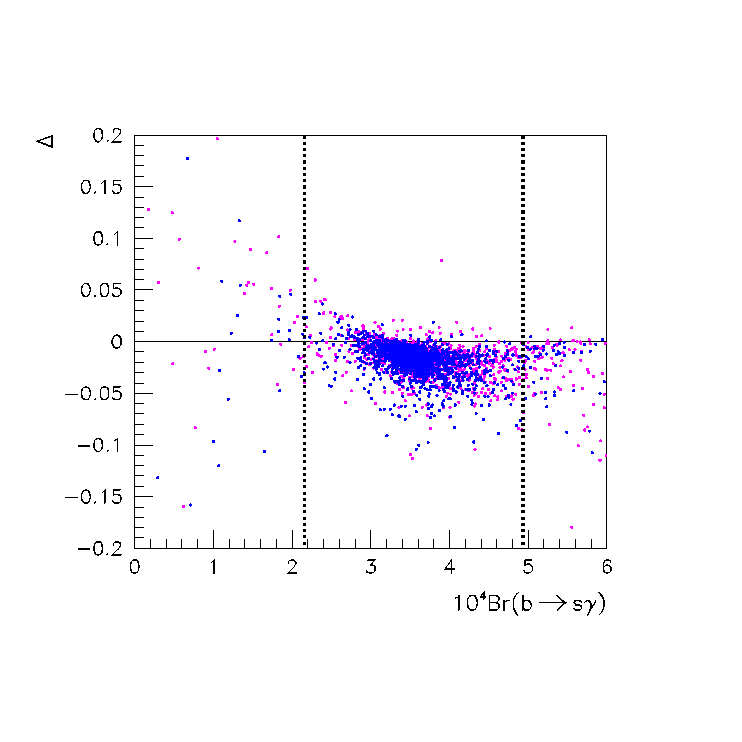
\includegraphics[width=8cm]{bsgiso.eps}
\vspace{-.3cm}
\caption{ Relative difference for $B(\bar{B}\rightarrow s\gamma)$ between micromegas$2.4$ and superIso$3.1$.
the vertical lines show the $3\sigma$ experimentally measured value.
}
\end{figure}


\begin{thebibliography}{}



%\cite{Belanger:2001fz}
\bibitem{Belanger:2001fz}
  G.~Belanger, F.~Boudjema, A.~Pukhov and A.~Semenov,
  %``micrOMEGAs: A program for calculating the relic density in the MSSM,''
  Comput.\ Phys.\ Commun.\  {\bf 149} (2002) 103
  [arXiv:hep-ph/0112278].
  %%CITATION = CPHCB,149,103;%%

%\cite{Belanger:2004yn}
\bibitem{Belanger:2004yn}
  G.~Belanger, F.~Boudjema, A.~Pukhov and A.~Semenov,
  %``micrOMEGAs: Version 1.3,''
  Comput.\ Phys.\ Commun.\  {\bf 174} (2006) 577
  [arXiv:hep-ph/0405253].
  %%CITATION = CPHCB,174,577;%%

%\cite{Belanger:2006is}
\bibitem{Belanger:2006is}
  G.~Belanger, F.~Boudjema, A.~Pukhov and A.~Semenov,
  %``micrOMEGAs2.0: A program to calculate the relic density of dark matter  in
  %a generic model,''
  Comput.\ Phys.\ Commun.\  {\bf 176} (2007) 367
  [arXiv:hep-ph/0607059].
  %%CITATION = CPHCB,176,367;%%

%\cite{Belanger:2008sj}
\bibitem{Belanger:2008sj}
  G.~Belanger, F.~Boudjema, A.~Pukhov and A.~Semenov,
  %``Dark matter direct detection rate in a generic model with micrOMEGAs2.2,''
  Comput.\ Phys.\ Commun.\  {\bf 180} (2009) 747
  [arXiv:0803.2360 [hep-ph]].
  %%CITATION = CPHCB,180,747;%%



\bibitem{Belanger:2010gh}
  G.~Belanger, F.~Boudjema, P.~Brun, A.~Pukhov, S.~Rosier-Lees, P.~Salati and A.~Semenov,
  %``Indirect search for dark matter with micrOMEGAs2.4,''
  arXiv:1004.1092 [hep-ph].
  %%CITATION = ARXIV:1004.1092;%%
  
  \bibitem{Belanger:2013oya}
  G.~Belanger, F.~Boudjema, A.~Pukhov and A.~Semenov,
  %``micrOMEGAs3.1 : a program for calculating dark matter oservables,''
  arXiv:1305.0237 [hep-ph].
  
  \bibitem{Belyaev:2006jh}
  A.~Belyaev, C.~-R.~Chen, K.~Tobe and C.~-P.~Yuan,
  %``Phenomenology of littlest Higgs model with $T^-$ parity: including effects of $T^-$ odd fermions,''
  Phys.\ Rev.\ D {\bf 74} (2006) 115020
  [hep-ph/0609179].
  
  \bibitem{Barbieri:2006dq}
  R.~Barbieri, L.~J.~Hall and V.~S.~Rychkov,
  %``Improved naturalness with a heavy Higgs: An Alternative road to LHC physics,''
  Phys.\ Rev.\ D {\bf 74} (2006) 015007
  [hep-ph/0603188].


  \bibitem{Belanger:2012vp}
  G.~Belanger, K.~Kannike, A.~Pukhov and M.~Raidal,
  %``Impact of semi-annihilations on dark matter phenomenology - an example of Z_N symmetric scalar dark matter,''
  JCAP {\bf 1204} (2012) 010
  [arXiv:1202.2962 [hep-ph]].

  \bibitem{Hindmarsh:2005ix}
  M.~Hindmarsh and O.~Philipsen,
  %``WIMP dark matter and the QCD equation of state,''
  Phys.\ Rev.\ D {\bf 71} (2005) 087302
  [hep-ph/0501232].


\bibitem{Beringer:1900zz}
  J.~Beringer {\it et al.}  [Particle Data Group Collaboration],
  %``Review of Particle Physics (RPP),''
  Phys.\ Rev.\ D {\bf 86} (2012) 010001.

\bibitem{Zhao:1995cp}
  H.~Zhao,
  %``Analytical models for galactic nuclei,''
  Mon.\ Not.\ Roy.\ Astron.\ Soc.\  {\bf 278} (1996) 488
  [astro-ph/9509122].

\bibitem{Lavalle:2006vb}
  J.~Lavalle, J.~Pochon, P.~Salati and R.~Taillet,
  %``Clumpiness of dark matter and positron annihilation signal: computing the odds of the galactic lottery,''
  Astron.\ Astrophys.\  {\bf 462} (2007) 827
  [astro-ph/0603796].
  %%CITATION = ASTRO-PH/0603796;%%

%\cite{Allanach:2008qq}
\bibitem{Allanach:2008qq}
  B.~Allanach {\it et al.},
  %``SUSY Les Houches Accord 2,''
  Comput.\ Phys.\ Commun.\  {\bf 180} (2009) 8
  [arXiv:0801.0045 [hep-ph]].
  %%CITATION = CPHCB,180,8;%%

%\cite{Hugonie:2007vd}
\bibitem{Hugonie:2007vd}
  C.~Hugonie, G.~Belanger and A.~Pukhov,
  %``Dark Matter in the Constrained NMSSM,''
  JCAP {\bf 0711} (2007) 009
  [arXiv:0707.0628 [hep-ph]].
  %%CITATION = JCAPA,0711,009;%%






%\cite{Belanger:2006qa}
\bibitem{Belanger:2006qa}
  G.~Belanger, F.~Boudjema, S.~Kraml, A.~Pukhov and A.~Semenov,
  %``Relic density of neutralino dark matter in the MSSM with CP violation,''
  Phys.\ Rev.\  D {\bf 73} (2006) 115007
  [arXiv:hep-ph/0604150].
  %%CITATION = PHRVA,D73,115007;%%



%\cite{Belanger:2005kh}
\bibitem{Belanger:2005kh}
  G.~Belanger, F.~Boudjema, C.~Hugonie, A.~Pukhov and A.~Semenov,
  %``Relic density of dark matter in the NMSSM,''
  JCAP {\bf 0509} (2005) 001
  [arXiv:hep-ph/0505142].
  %%CITATION = JCAPA,0509,001;%%




%\cite{Skands:2003cj}
\bibitem{Skands:2003cj}
  P.~Skands {\it et al.},
  %``SUSY Les Houches accord: Interfacing SUSY spectrum calculators, decay
  %packages, and event generators,''
  JHEP {\bf 0407} (2004) 036
  [arXiv:hep-ph/0311123].
  %%CITATION = JHEPA,0407,036;%%




%\cite{Pukhov:2004ca}
\bibitem{Pukhov:2004ca}
  A.~Pukhov,
  %``CalcHEP 3.2: MSSM, structure functions, event generation, batchs, and
  %generation of matrix elements for other packages,''
  arXiv:hep-ph/0412191.
  %%CITATION = HEP-PH/0412191;%%

   \bibitem{Belyaev:2012qa}
   A.~Belyaev, N.~D.~Christensen and A.~Pukhov,
   %``CalcHEP 3.4 for collider physics within and beyond the Standard Model,''
   Comput.\ Phys.\ Commun.\  {\bf 184} (2013) 1729
   [arXiv:1207.6082 [hep-ph]].

%\cite{Semenov:2008jy}
\bibitem{Semenov:2008jy}
  A.~Semenov,
  %``LanHEP - a package for the automatic generation of Feynman rules in field
  %theory. Version 3.0,''
  Comput.\ Phys.\ Commun.\  {\bf 180} (2009) 431
  [arXiv:0805.0555 [hep-ph]].
  %%CITATION = CPHCB,180,431;%%

%\cite{Belanger:2007dx}
\bibitem{Belanger:2007dx}
  G.~Belanger, A.~Pukhov and G.~Servant,
  %``Dirac Neutrino Dark Matter,''
  JCAP {\bf 0801} (2008) 009
  [arXiv:0706.0526 [hep-ph]].
  %%CITATION = JCAPA,0801,009;%%

\bibitem{Eidelman:2004wy}
  S.~Eidelman {\it et al.}  [Particle Data Group],
  %``Review of particle physics,''
  Phys.\ Lett.\  B {\bf 592} (2004) 1.
  %%CITATION = PHLTA,B592,1;%%



%\cite{Ellwanger:2006rn}
\bibitem{Ellwanger:2006rn}
  U.~Ellwanger and C.~Hugonie,
  %``NMSPEC: A Fortran code for the sparticle and Higgs masses in the NMSSM with
  %GUT scale boundary conditions,''
  Comput.\ Phys.\ Commun.\  {\bf 177} (2007) 399
  [arXiv:hep-ph/0612134].
  %%CITATION = CPHCB,177,399;%%
  
  \bibitem{Ellwanger:2005dv}
  U.~Ellwanger and C.~Hugonie,
  %``NMHDECAY 2.0: An Updated program for sparticle masses, Higgs masses,
  %couplings and decay widths in the NMSSM,''
  Comput.\ Phys.\ Commun.\  {\bf 175} (2006) 290
  [arXiv:hep-ph/0508022].
  %%CITATION = CPHCB,175,290;%%
  
  \bibitem{Domingo:2007dx}
  F.~Domingo and U.~Ellwanger,
  %``Updated Constraints from $B$ Physics on the MSSM and the NMSSM,''
  JHEP {\bf 0712} (2007) 090
  [arXiv:0710.3714 [hep-ph]].
  %%CITATION = JHEPA,0712,090;%%
  
  
  \bibitem{Lee:2003nta}
  J.~S.~Lee, A.~Pilaftsis, M.~S.~Carena, S.~Y.~Choi, M.~Drees, J.~R.~Ellis and C.~E.~M.~Wagner,
  %``CPsuperH: A computational tool for Higgs phenomenology in the minimal
  %supersymmetric standard model with explicit CP violation,''
  Comput.\ Phys.\ Commun.\  {\bf 156} (2004) 283
  [arXiv:hep-ph/0307377].
  %%CITATION = CPHCB,156,283;%%

\bibitem{Lee:2007gn}
  J.~S.~Lee, M.~Carena, J.~Ellis, A.~Pilaftsis and C.~E.~M.~Wagner,
  %``CPsuperH2.0: an Improved Computational Tool for Higgs Phenomenology in the
  %MSSM with Explicit CP Violation,''
  Comput.\ Phys.\ Commun.\  {\bf 180} (2009) 312
  [arXiv:0712.2360 [hep-ph]].
  %%CITATION = CPHCB,180,312;%%
  
  \bibitem{CPSUPERH}
  J.S.~Lee, A. Pilaftsis, M.~Carena, S.Y.~Choi, M.~Drees, J.~Ellis, C. Wagner,\\
  \verb|http://www.hep.man.ac.uk/u/jslee/CPsuperH.html|.
  
  \bibitem{nmssmtools}
  U.~Ellwanger, J.~Gunion, C.~Hugonie,\\
  \verb|http://www.th.u-psud.fr/NMHDECAY/nmssmtools.html|.


\bibitem{Numerical}
W.~H.~Press, S.~A.~Teukolsky,
W.~T.~Vetterling and  B.~P.~ Flannery,  
"Numerical Recipes: The Art of Scientific Computing'', Cambridge University
Press (2007).

%\cite{Mahmoudi:2010iz}
\bibitem{Mahmoudi:2010iz}
  F.~Mahmoudi {\it et al.},
  %`Flavour Les Houches Accord: Interfacing Flavour related Codes,''
  arXiv:1008.0762 [hep-ph].
  %%CITATION = ARXIV:1008.0762;%%

%\cite{Arbey:2011zz}
\bibitem{Arbey:2011zz}
  A.~Arbey and F.~Mahmoudi,
  %`SuperIso Relic v3.0: A program for calculating relic density and flavour
  %physics observables: Extension to NMSSM,''
  Comput.\ Phys.\ Commun.\  {\bf 182} (2011) 1582.
  %%CITATION = CPHCB,182,1582;%%

\bibitem{Misiak:2006zs}
  M.~Misiak, H.~M.~Asatrian, K.~Bieri, M.~Czakon, A.~Czarnecki, T.~Ewerth, A.~Ferroglia, P.~Gambino {\it et al.},
  %``Estimate of B(anti-B ---> X(s) gamma) at O(alpha(s)**2),''
  Phys.\ Rev.\ Lett.\  {\bf 98 } (2007)  022002.
  [hep-ph/0609232].

\bibitem{Misiak:2006ab}
  M.~Misiak, M.~Steinhauser,
  %``NNLO QCD corrections to the anti-B ---> X(s) gamma matrix elements using interpolation in m(c),''
  Nucl.\ Phys.\  {\bf B764 } (2007)  62-82.
  [hep-ph/0609241].

\bibitem{Gambino:2008fj}
  P.~Gambino, P.~Giordano,
  %``Normalizing inclusive rare B decays,''
  Phys.\ Lett.\  {\bf B669 } (2008)  69-73.
  [arXiv:0805.0271 [hep-ph]].

\bibitem{Yao:2006px}
  W.~M.~Yao {\it et al.} [ Particle Data Group Collaboration ],
  %``Review of Particle Physics,''
  J.\ Phys.\ G {\bf G33 } (2006)  1-1232.

\bibitem{Nakamura:2010zzi}
  K.~Nakamura {\it et al.} [ Particle Data Group Collaboration ],
  %``Review of particle physics,''
  J.\ Phys.\ G {\bf G37 } (2010)  075021.
  
%\cite{Jungman:1995df}
\bibitem{Jungman:1995df}
  G.~Jungman, M.~Kamionkowski and K.~Griest,
  %``Supersymmetric dark matter,''
  Phys.\ Rept.\  {\bf 267} (1996) 195
  [hep-ph/9506380].
  %%CITATION = HEP-PH/9506380;%%
%\cite{Cirelli:2005gh}
\bibitem{Cirelli:2005gh}
  M.~Cirelli, N.~Fornengo, T.~Montaruli, I.~A.~Sokalski, A.~Strumia and
F.~Vissani,
  %``Spectra of neutrinos from dark matter annihilations,''
  Nucl.\ Phys.\ B {\bf 727} (2005) 99
   [Erratum-ibid.\ B {\bf 790} (2008) 338]
  [hep-ph/0506298].
  %%CITATION = HEP-PH/0506298;%%


%\cite{Erkoca:2009by}
\bibitem{Erkoca:2009by}
  A.~E.~Erkoca, M.~H.~Reno and I.~Sarcevic,
  %``Muon Fluxes From Dark Matter Annihilation,''
  Phys.\ Rev.\ D {\bf 80} (2009) 043514
  [arXiv:0906.4364 [hep-ph]].
  %%CITATION = ARXIV:0906.4364;%%

\bibitem{Maurin:2006hy}
  D.~Maurin, R.~Taillet and C.~Combet,
  %``Approximate formulae for exotic GCR anti-protons and anti-deuterons:
  % Fluxes and astrophysical uncertainties,''
  %Submitted to: Phys.Rev.D
  [astro-ph/0609522].

%\cite{Belanger:2014bga}
\bibitem{Belanger:2014bga}
  G.~B\'elanger, K.~Kannike, A.~Pukhov and M.~Raidal,
  %``Minimal semi-annihilating $\mathbb{Z}_N$ scalar dark matter,''
  JCAP {\bf 1406} (2014) 021
  [arXiv:1403.4960 [hep-ph]].
  %%CITATION = ARXIV:1403.4960;%%
  %1 citations counted in INSPIRE as of 17 Jul 2014


   \bibitem{Bechtle:2013xfa}
   P.~Bechtle, S.~Heinemeyer, O.~St\"al, T.~Stefaniak and G.~Weiglein,
   %``HiggsSignals: Confronting arbitrary Higgs sectors with measurements at the Tevatron and the LHC,''
   arXiv:1305.1933 [hep-ph].
 
   \bibitem{Bechtle:2013wla}
   P.~Bechtle, O.~Brein, S.~Heinemeyer, O.~St\"al, T.~Stefaniak, G.~Weiglein and K.~E.~Williams,
   %``HiggsBounds-4: Improved Tests of Extended Higgs Sectors against Exclusion Bounds from LEP, the Tevatron and the LHC,''
   arXiv:1311.0055 [hep-ph].

\end{thebibliography}
\end{document}

